% Format teze zasnovan je na paketu memoir
% http://tug.ctan.org/macros/latex/contrib/memoir/memman.pdf ili
% http://texdoc.net/texmf-dist/doc/latex/memoir/memman.pdf
% 
% Prilikom zadavanja klase memoir, navedenim opcijama se podešava 
% veličina slova (12pt) i jednostrano štampanje (oneside).
% Ove parametre možete menjati samo ako pravite nezvanične verzije
% mastera za privatnu upotrebu (na primer, u b5 varijanti ima smisla 
% smanjiti 
\documentclass[12pt,oneside]{memoir}
\sloppy
\usepackage{cmap}

% Paket koji definiše sve specifičnosti mastera Matematičkog fakulteta
\usepackage{matfmaster}
\usepackage{hyperref}
\hypersetup{colorlinks,linkcolor={blue},citecolor={blue},urlcolor={blue}}

%\usepackage[T1]{fontenc}
\usepackage{xcolor}
\usepackage{color}
\usepackage{listings}

\definecolor{dkgreen}{rgb}{0,0.6,0}
\definecolor{gray}{rgb}{0.5,0.5,0.5}
\definecolor{mauve}{rgb}{0.58,0,0.82}

\lstset{
language=Scala,
basicstyle=\small\ttfamily,
columns=fullflexible,
keywords=[2]{fail},
keywords=[3]{pass},
keywordstyle={\color{blue!80!black}},
keywordstyle=[2]{\color{red!80!black}},
keywordstyle=[3]{\color{green!50!black}},
commentstyle=\color{dkgreen},
numberstyle=\tiny\color{gray},
stringstyle=\color{mauve},
showstringspaces=false,
tabsize=3,
breaklines=true,
breakatwhitespace=true
}

%\usepackage{minted}
%
% Podrazumevano pismo je ćirilica.
%   Ako koristite pdflatex, a ne xetex, sav latinički tekst na srpskom jeziku
%   treba biti okružen sa \lat{...} ili \begin{latinica}...\end{latinica}.
%
% Opicija [latinica]:
%   ako želite da pišete latiniciom, dodajte opciju "latinica" tj.
%   prethodni paket uključite pomoću: \usepackage[latinica]{matfmaster}.
%   Ako koristite pdflatex, a ne xetex, sav ćirilički tekst treba biti
%   okružen sa \cir{...} ili \begin{cirilica}...\end{cirilica}.
%
% Opcija [biblatex]:
%   ako želite da koristite reference na više jezika i umesto paketa
%   bibtex da koristite BibLaTeX/Biber, dodajte opciju "biblatex" tj.
%   prethodni paket uključite pomoću: \usepackage[biblatex]{matfmaster}
%
% Opcija [b5paper]:
%   ako želite da napravite verziju teze u manjem (b5) formatu, navedite
%   opciju "b5paper", tj. prethodni paket uključite pomoću: 
%   \usepackage[b5paper]{matfmaster}. Tada ima smisla razmisliti o promeni
%   veličine slova (izmenom opcije 12pt na 11pt u \documentclass{memoir}).
%
% Naravno, opcije je moguće kombinovati.
% Npr. \usepackage[b5paper,biblatex]{matfmaster}

% Pomoćni paket koji generiše nasumičan tekst u kojem se javljaju sva slova
% azbuke (nema potrebe koristiti ovo u pravim disertacijama)
\usepackage{pangrami}
\usepackage[utf8]{inputenc}
\usepackage[english, serbian]{babel}
\usepackage{amsthm}
\usepackage{graphicx}
%\usepackage{caption}
\usepackage{subfig}
%\usepackage{subfigure}
\setcounter{tocdepth}{3}
\setsecnumdepth{subsubsection}

%\usepackage{tikz}
% Datoteka sa literaturom u BibTex tj. BibLaTeX/Biber formatu
\bib{tezaBib}

% Ime kandidata na srpskom jeziku (u odabranom pismu)
\autor{Aна Д. Митровић}
% Naslov teze na srpskom jeziku (u odabranom pismu)
\naslov{Примена Скале у паралелизацији расплинутог тестирања}
% Godina u kojoj je teza predana komisiji
\godina{2019}
% Ime i afilijacija mentora (u odabranom pismu)
\mentor{др Милена Вујошевић Јаничић, доцент\\ Универзитет у Београду, Математички факултет}
% Ime i afilijacija prvog člana komisije (u odabranom pismu)
\komisijaA{др Саша Малков, ванредни професор\\ Универзитет у Београду, Математички факултет}
% Ime i afilijacija drugog člana komisije (u odabranom pismu)
\komisijaB{др Александар Картељ, доцент\\ Универзитет у Београду, Математички факултет}
% Ime i afilijacija trećeg člana komisije (opciono)
% \komisijaC{}
% Ime i afilijacija četvrtog člana komisije (opciono)
% \komisijaD{}
% Datum odbrane (obrisati ili iskomentarisati narednu liniju ako datum odbrane nije poznat)
\datumodbrane{2019.}

% Apstrakt na srpskom jeziku (u odabranom pismu)
\apstr{Примена софтвера из дана у дан постаје све шира и од софтвера се све више очекује. У оквиру најразличитијих очекивања, посебно се издвајају исправност и ефикасност софтвера, две карактеристике које се готово подразумевају и не зависе од намене софтверског производа. Да би се проверила исправност софтвера користе се различите технике тестирања. За остваривање ефикасности, све чешће се користе технике конкурентног програмирања. Оне нам омогућавају боље искоришћавање модерног хардвера тј. вишејезгарних процесора. У овом раду представљене су технике тестирања софтвера и имплементирана је техника аутоматског тестирања робусности софтвера која се назива расплинуто тестирање. Овом техником тестирани су читачи датотека у формату \textit{PDF}. Ради постизања ефикасности, тестирање се обавља конкурентно и имплементирано је у програмском језику Скала.  Поред увода у тестирање софтвера и конкурентно програмирање, циљ овог рада је и упознавање карактеристика језика Скала. Скала је језик опште намене који подржава две парадигме програмирања - објектну и функционалну парадигму. У раду је фокус на напреднијим карактеристикама језика, оним које су погодне за конкурентно програмирање. 
}

% Ključne reči na srpskom jeziku (u odabranom pismu)
\kljucnereci{програмски језик Скала, конкурентно програмирање, паралелно програмирање, расплинуто тестирање софтвера}

\usepackage{tikz}
\newcommand{\quem}{\tikz[baseline=(wi.base)]{\node[fill=black,rotate=45,inner sep=.1ex, text height=1.8ex, text width=1.8ex] {};%
\node[ font=\color{white}] (wi) {?};}}

\usepackage{makecell}
\renewcommand\theadfont{\bfseries\sffamily}

\begin{document}
% ==============================================================================
% Uvodni deo teze
\frontmatter
% ==============================================================================
% Naslovna strana
\naslovna
% Strana sa podacima o mentoru i članovima komisije
\komisija
% Strana sa podacima o disertaciji na srpskom jeziku
\apstrakt
% Sadržaj teze
\tableofcontents*

% ==============================================================================
% Glavni deo teze
\mainmatter
% ==============================================================================

% ------------------------------------------------------------------------------
\chapter{Увод}

У области рачунарства напредак нових технологија је веома брз због потреба за све захтевнијим системима који су присутни у нашем свакодневном животу. Константно се развијају и софтвер и хардвер који омогућавају развој сигурнијих, бржих и ефикаснијих апликација разних намена. Неке од најважних карактеристика данашњих рачунара су конкурентно и паралелно извршавање процеса. Данас се углавном програми извршавају на вишејезгарним процесорима, који могу значајно да допринесу побољшању перформанси програма. 

Функционална парадигма програмирања има особине које су погодне за паралелно програмирање. Дељење меморије међу нитима и руковање променљивим подацима изискују синхронизацију и закључавање, што је подложно грешкама. Транспарентност референци и коришћење непроменљивих података су особине функционалних програмских језика које олакшавају паралелизацију задатака. Програмски језик Скала је објектно оријентисан језик који подржава функционално програмирање, због чега може искористити предности функционалне парадигме. Скала искоришћава и предности објектне парадигме, па је погодна за програме различитих намена. Поред тога, компатибилна је са Јавом што омогућава лакше привикавање програмера на нови језик.

Иако Скала подржава функционално програмирање, у раду су проблеми модела дељења меморије превазиђени другачијим стилом паралелног програмирања. Обрађен је модел размене порука под називом Актер. Коришћена је библиотека \textit{Akka}, која је заједничка за Јаву и Скалу. Као задатак који треба паралелизовати одабрана је техника тестирања робусности софтвера под називом расплинуто тестирање\footnote{Термин "расплинуто" се не односи на расплинуте (енг. \textit{fuzzy}) логике и скупове.}. Ова техника се базира на генерисању великог броја правилних и неправилних улаза у програм како би што више различитих случајева било испитано. Због генерисања различитих улаза, расплинуто тестирање је веома погодно за примену паралелизације тако што свака компонента тестирања паралелно може генерисати улаз за програм. У овом раду су тестирани читачи датотека у формату \textit{PDF}, тако да су улази у програм такве датотеке.

Још један разлог одабира технике тестирања за задатак који треба паралелизовати је велики значај тестирања софтвера. Поред саме имплементације програма јако је важно тестирати програм. Иако само тестирање не може доказати исправност софтвера, оно игра велику улогу у проналажењу и исправљању грешака чиме се повећава поузданост софтверa. Због тога су у раду обухваћене и основе тестирања софтвера.

Рад је организован на следећи начин. У глави \ref{chp:skala} детаљно је описан програмски језик Скала. Описане су његове опште карактеристике (поглавље \ref{sec:opsteKarakt}) са посебним акцентом на функционални део језика (поглавље \ref{sec:funkDeoJezika}). Детаљно је описан концепт паралелизма (поглавље \ref{sec:paralelizam}) и библиотека \textit{Akka} (поглавље \ref{sec:akka}). У глави \ref{chp:rasplTestiranje} је описана техника расплинутог тестирања. Поглавље \ref{sec:osnoveTestiranja} садржи основе тестирања софтвера, а поглавље \ref{sec:osnoveRasplTestiranja} основе расплинутог тестирања. Врсте програма расплинутог тестирања описане су у поглављу \ref{sec:vrsteProRaspTest}, а расплинуто тестирање формата датотека описано је у поглављу \ref{sec:rasTestFormFajl}. Структура датотека у формату \textit{PDF} описана је у глави \ref{chp:pdfStruktura}. Описани су објекти датотека (поглавље \ref{sec:objektiPDF}), организација датотека (поглавље \ref{sec:organizacijaDatotekaPDF}) и њихово ажурирање (поглавље \ref{sec:azuriranje}). У глави \ref{chp:implementacija} описана је имплементација програма за расплинуто тестирање. Описани су улазни параметри програма (поглавље \ref{sec:ulazniParametri}), организација програма (поглавље \ref{sec:orgProg}), објекти Актер (поглавље \ref{sec:actorObj}), креирање улазних датотека (поглавље \ref{sec:kreiranjeDat}) и постигнути резултати (поглавље \ref{sec:rez}). У глави \ref{chp:zakljucak} дати су закључци рада. 

% ------------------------------------------------------------------------------

% ------------------------------------------------------------------------------
\chapter{Програмски језик Скала}
\label{chp:skala}
% ------------------------------------------------------------------------------

Скала је језик опште намене настао 2003. године са циљем да превазиђе ограничења програмског језика Јава комбиновањем објектно оријентисанe и функционалнe програмске парадигме. Мотивација иза овакве идеје је не ограничавати се на једну од ових парадигми и њених предности већ искористити најбоље из оба света. Управо због овакве комбинације парадигми, Скала је веома погодна за решавање различитих врста проблема, почевши од малих незахтевних скриптова па све до великих компликованих система. На основу ове прилагодљивости је и добила своје име: реч "скала" означава "скалабилан језик" (енг. \textit{scalable language}), односно језик који ће се прилагођавати и расти заједно са потребама система \cite{progInScala}.
\par Творац Скале је Мартин Одерски (нем. \textit{Martin Odersky}) (1958-), немачки научник и професор на универзитету \textit{EPFL} (École Polytechnique Fédérale de Lausanne) у Лозани у Швајцарској. Још док је био студент, имао је жељу да напише језик који ће подржавати објектну и функционалну парадигму, говорећи да су ове две парадигме само две стране истог новчића. Желео је да се тај језик преводи у Јава бајт к\^{о}д али и да превазиђе ограничења језика Јава. Први резултат оваквог његовог рада је био језик \textit{Funnel}, који због свог минималистичког дизајна није заживео. Затим је настала Скала, коју је професор Одерски развијао од 2001. године заједно са својом групом на универзитету \textit{EPFL}. Познат је и по другим радовима, као што je имплементација компајлера \textit{GJ} (\textit{Generic Java}) који је постао основа компајлера \textit{javac} \cite{MartinEpfl, ScalaHistory}.

\section{Опште карактеристике}
\label{sec:opsteKarakt}

Прилагођавање потребама система је у Скали лако и веома удобно. Томе доприноси могућност програмера да дефинише библиотеке које су веома лаке за коришћење и које се користе једнако интуитивно као и библиотеке које се већ налазе у самом језику. У наставку су наведене неке од најважнијих особина Скале које доприносе њеној "скалабилности" \cite{progInScala}:

\begin{description}
\item \textbf{Компатибилност са Јавом} Скала није сама по себи продужење Јаве, али је потпуно компатибилна са њом: њен изворни к\^{о}д се преводи у Јава бајт к\^{о}д који се извршава на Јава виртуелној машини. У коду написаном у Скали је омогућено коришћење библиотека, класа, интерфејса, метода, поља и типова језика Јава. Омогућено је и обрнуто, позивање кода написаног у Скали из Јаве, мада се оно ређе користи. Такође, у Скали је омогућена лакша и лепша употреба типова језика Јава уз помоћ имплицитне конверзије. Тиме је омогућена употреба метода за манипулацију типовима које има Скала. Компатибилност олакшава програмерима лакши прелазак из Јаве у Скалу јер нису принуђени да се одједном одрекну написаног кода у Јави.

Корен Скале није само језик Јава, иако је Јава имала највећи утицај у њеном стварању. Идеје и концепти из разних језика, како објектно оријентисаних тако и функционално оријентисаних, су инспирисали развој Скале. Међу њима су језици: \textit{C\#}  од кога је Скала преузела синтаксне конвенције, \textit{Erlang} чије идеје су сличне идејама конкурентности базиране на моделу Актер и други: \textit{C}, \textit{C++},  \textit{Smalltalk}, \textit{Ruby}, \textit{Haskell}, \textit{SML}, \textit{F\#} итд.

\item \textbf{Објектно оријентисана парадигма} Писање програма и смештање података и њихових својстава у класе и објекте тих класа је веома популарно и интуитивно програмерима. Скала је то задржала, притом мало изменивши концепт. У многим језицима, укључујући и Јаву, дозвољене су вредности које нису објекти или које нису у склопу објекта. То могу бити примитивне вредности у Јави или статичка поља и методи. Скала то не дозвољава и зато је објектно оријентисан језик у \textit{чистој форми}: "Свака вредност је објекат и свака операција је позив метода" \cite{progInScala}. Елегантан начин коришћења метода налик на операције је једна од особина Скале које је чине пријатном за коришћење.

\item \textbf{Концизност} К\^{о}д написан у Скали има тенденцију да буде краћи од кода написаног у Јави. Чак се процењује да к\^{о}д написан у Скали има барем два пута мање линија кода од одговарајућег кода написаног у Јави. Постоје и екстремни случајеви где је број линија и десет пута мањи. Ова особина није значајна само због тога што знатно олакшава програмирање, већ олакшава читање кода и откривање грешака. Ово је нешто што одликује саму синтаксу језика, а веома помажу и разне библиотеке које имају већ имплементиране многе функције које врше послове са којима се често сусрећемо. Лако се имплементирају и касније употребљавају библиотеке које сами напишемо. Такође, у Скали је подржано аутоматско закључивање типова (енг. \textit{type inference}), што омогућава изостављање навођења неких типова, што резултује краћим и често читљивијим кодом.

\item \textbf{Висок ниво} Скала је погодна за велике и комплексне системе и може се прилагодити њиховим захтевима подижући ниво апстракције у коду. Омогућен је много једноставнији и краћи начин кодирања разних проблема. Рецимо, уместо да пролазимо кроз ниску карактера карактер по карактер користећи петљу, у Скали се то може урадити у једној линији кода помоћу \textit{предиката} тј.  \textit{функцијских литерала} који су детаљније објашњени у поглављу \ref{sec:funkDeoJezika}. К\^{о}д написан у Скали је разумљивији и мање комплексан, што је важно јер је систем који се имплеметира сам по себи комплексан.

\item \textbf{Статичка типизираност} Скала је статички типизиран језик што значи да се типови података који су коришћени знају у време компилације. Неки сматрају ово маном, као и да је навођење типова сувишно поред техника тестирања софтвера као што је нпр. тестирање јединица кода (енг. \textit{unit testing}). Ипак, у Скали је статичка типизираност напреднија. Довољно је навести тип само једном уместо више пута. Понављање нарушава читљивост кода, али је ипак у неким језицима неопходно. Због оваквих понављања, многи се одрекну предности статички типизираних језика као што су: детектовање разних грешака у време компилације, лакше рефакторисање кода и коришћење типова као вида документације.

\item \textbf{Способности} Скала уводи појам способности (енг. \textit{trait}) које делe карактеристике са интерфејсима и наслеђивањем класа у Јави. У способностима као и у интерфејсима можемо декларисати методе, али и дефинисати поља и конкретне методе што није могуће у интерфејсима. Променљиве омогућавају чување стања а методе дефинисање одређеног понашања. То чини способности богатијим од интерфејса. Кажемо да се способности "спајају" у класе (енг. \textit{mix in}). У једну класу је могуће спојити више способности.

Спајање се може остварити кључном речју \textbf{extends} и у том случају класа наслеђује наткласу способности. У случају да желимо да класа наследи неку другу класу, онда помоћу \textit{extends} наводимо наткласу а способности спајамо помоћу \textbf{with} као што је илустровано у наредном примеру \cite{progInScala}: 

\begin{lstlisting}[language=Scala]
class Animal
trait HasLegs
trait Philosophical
/* Natklasa "Animal" i spojena svojstva "HasLegs" i "Philosophical" */
class Frog extends Animal with HasLegs with Philosophical {
	/* ... */
}
\end{lstlisting}

Највећа разлика између класе и способности односи се на позивање метода наткласе помоћу поља \textit{super}. На пример, позивом метода \textit{super.toString()} у случају класе, тачно се зна који ће метод \textit{toString()} бити позван јер се зна наткласа дате класе. У случају способности, не можемо знати на шта се овај позив односи јер то директно зависи од класе у коју ће дата способност бити спојена, као и од претходно спојених способности. То значи да се позиви \textit{super} одређују \textit{динамички}. Свака спојена способност може позвати метод претходно спојене способности. Ово омогућава класама да стекну различито понашање у зависности од редоследа спојених способности. Помоћу малог броја дефинисаних способности може се постићи много различитих циљева комбиновањем редоследа спајања.

\end{description}
\par Иако је Скала објектно оријентисани језик, она има елементе функционалне парадигме и подржава чисто функционално програмирање. Функционална природа Скале је детаљно објашњена у следећем поглављу.

% --------
\section{Функционални део језика}
\label{sec:funkDeoJezika}

Функционална парадигма се развија од 1950-тих година. Чисто функционални програмски језик може да се
посматра и као математичка формализација алгоритма (може и обрнуто). Примери таквих формализама су \textit{ламбда рачун} (енг. \textit{$\lambda$-calculus}) и комбинаторна логика. Ламбда рачун представља математичку апстракцију и формализам за описивање функција и њихово израчунавање. Њега је увео Алонзо Черч (енг. \textit{Alonzo Church}) 1930-тих година а Алан Тјуринг (енг. \textit{Alan Turing}) је 1937. године показао да је експресивност ламбда рачуна еквивалентна експресивности Тјурингових машина. Иако је ламбда рачун првобитно развијен само за потребе математике, данас се он сматра првим функционалним језиком. Други модел рачунања који је утицао на функционалне програмске језике, комбинаторну логику, створили су Мојсеј Шејнфинкел (рус. \textit{Моисей Шейнфинкель}) и Хаскел Кари (енг. \textit{Haskell Curry}) 1924. године са циљем да елиминишу употребу променљивих у математичкој логици \cite{funkMilena, funkMalkov, lambdaRacun, history}.
\par Најстарији виши функционални програмски језик је \textit{LISP} који је пројектовао Џон Макарти (енг. \textit{John McCarthy}) на институту МИТ (Масачусетски технолошки институт) 1958. године. Након тога се полако развијају и други функционални језици као што су \textit{ISWIM}, \textit{FP}, \textit{Scheme}, \textit{ML}, \textit{Miranda}, \textit{Erlang}, \textit{SML}, \textit{Haskell}, \textit{OCAML}, \textit{ F\#}, \textit{Elixir} итд. Поред функционалних језика постоје и језици који нису функционални али  у одређеној мери подржавају функционалне концепте или могу да их остваре на други начин, нпр. \textit{Java}, \textit{C}, \textit{C$++$}, \textit{C\#}, \textit{Python} \cite{funkMilena, history}.
\par Разлика између императивне и функционалне парадигме се може описати разликом у начину дефинисања појма програма и начину писања програма \cite{funkMalkov}:
\begin{itemize}
\item Императивна парадигма: 
\\Програм представља формално упутство о томе шта рачунар треба да ради да би урадио неки посао
\\Програм представља одговор на питање КАКО се нешто РАДИ
\item Функционална парадигма:
\\Програм представља формално објашњење онога што рачунар треба да израчуна
\\Програм представља одговор на питање ШТА се РАЧУНА
\end{itemize}
\par Функционални језици су веома блиски математичком начину размишљања због чега се и називају \textit{функционалним} језицима: њихове функције се понашају као функције у математичком смислу. О томе говоре следеће две карактеристике функционалних језика \cite{progInScala}: 
\par Прва карактеристика се односи на \textbf{"статус" функција}. У функционалним језицима функције су вредности \textit{првог реда}, тј. \textit{грађани првог реда}. То значи да се променљиве чије су вредности функције могу користити као променљиве других типова као што су нпр. цели, реални бројеви, ниске карактера итд. Ово омогућава коришћење функција на природан, концизан и читљив начин: као аргументе других функција, повратне вредности функција, њихово чување у променљивим, угњеждавање и слично. Другим речима, функције се креирају и прослеђују без икаквих рестрикција на које смо навикли у императивним језицима.
\par У Скали можемо користити локалне (угњеждене) функције које су често веома мале и лако се комбинују како би заједно заокружиле један већи посао. Ово одговара функционалном стилу који промовише следећу идеју: програм треба изделити на много мањих функција (целина) од којих свака има јасно дефинисан задатак.
\par Посебно су корисни и важни \textit{функцијски литерали} који представљају функције које могу бити неименоване и прослеђиване као обичне вредности. Функцијски литерали се у другим језицима називају "анонимне" или чешће "ламбда" функције. Назив "функцијски литерал" се користи за функције у изворном коду, а у време извршавања оне се називају \textit{функцијским вредностима} (разлика слична разлици између класа и објеката у објектно оријентисаним језицима). Функцијске вредности су објекти које можемо чувати у променљивама али су истовремено и функције које можемо позивати. Пример функцијског литерала који инкрементира цео број изгледа овако \cite{progInScala}:
\begin{lstlisting}[language=Scala]
var increase = (x: Int) => x + 1
increase(10)
\end{lstlisting}
Променљива \textit{increase} је објекат који садржи литерал и чија је вредност функција коју позивамо са аргументом 10.
\par Друга карактеристика се односи на \textbf{непостојање стања} које се иначе представља променљивама у програму. То значи да извршавање метода нема \textit{бочне ефекте}, односно да функције које позивамо не мењају податке "у месту" већ враћају нове вредности као резултате свог израчунавања. Уместо променљивих чија се стања ажурирају, користе се \textit{именоване вредности}. Именоване вредности се иницијализују само једном, а у Скали се дефинишу помоћу кључне речи \textbf{val}. Покушаj промене именоване вредности након што jе инициjализована резултирао би грешком. Поред именованих вредности, у Скали је дозвољено коришћење променљивих јер она није чист функционални језик. Променљиве се дефинишу кључном речjу \textbf{var}.

\par Непостојање стања има за последицу избацивање итеративних конструкција. Овакав приступ може испрва деловати необично и ограничавајуће, међутим све што се може остварити кроз итерације се може остварити и \textit{рекурзијом}. Класичан приступ функционалном програмирању подразумева употребу рекурзије, али треба напоменути да савремен приступ тежи да све рекурзије сведе на употребу стандардизованих функција вишег реда. Проблеми који захтевају чување и преношење променљивог стања некада имају компликовано решење у језицима који имају класичан приступ. Ипак, решење постоји, тако да се ово не сматра недостатком. Предност је у томе што не морамо пратити вредности променљивих и њихове промене што олакшава разумевање програма. Један програм у функционалном језику представља низ дефиниција и позива функција а његово извршавање је евалуација тих функција \cite{funkMilena}. Такође треба напоменути да је употреба рекурзије уобичајена за класичан приступ функционалном програмирању. Са друге стране, савремен приступ тежи да све рекурзије сведе на употребу стандардизованих функција вишег реда.
\par Као пример метода који нема бочне ефекте може послужити метод \textit{replace} који као аргументе добија ниску карактера и два карактера. Његов задатак је да у датој ниски замени сва појављивања једног карактера другим карактером. Он неће променити ниску коју је добио као аргумент, већ ће вратити нову која више нема појављивања датог карактера који смо заменили новим.  
\par Ова особина метода без бочних ефеката назива се \textbf{транспарентност референци} (енг. \textit{referential transparency}): позив метода можемо заменити његовим резултатом јер смо сигурни да ће при сваком позиву са истим вредностима аргумената вратити исти резултат. Пример:

\begin{lstlisting}[language=Scala]
val p = previous(90)
\end{lstlisting}
Свако појављивање променљиве \textit{p} можемо заменити изразом \textit{previous(90)}.

Вредност резултата не зависи од бочних ефеката и тренутног стања променљивих, већ само од вредности прослеђених аргумената. Због тога, редослед позива таквих метода није важан па може бити произвољан. За овакве методе кажемо да су референцијално транспарентни. Они су концизнији, читљивији и производе мање грешака јер немају бочне ефекте. Ипак, у Скали су присутни и бочни ефекти јер она није функционалан језик \cite{funkMilena}.
\par Чисто функционални језици (нпр. \textit{Haskel}, \textit{Miranda}) захтевају коришћење непроменљивих структура података, референцијално транспарентних метода и рекурзије. Други језици, као што су Скала, \textit{Python}, \textit{Ruby} охрабрују овакво програмирање али не условљавају програмера. Скала омогућава бирање начина за решавање проблема и нуди функционалне алтернативе за све императивне конструкције. На овај начин програмер се полако и без притиска навикава на другачији начин размишљања \cite{funkMilena, progInScala}.
\par Неке од карактеристика функционалних језика које Скала подржава су \cite{progInScala}:
\begin{description}
\item \textbf{Функције вишег реда} %strana 210
Функције вишег реда су оне које имају друге функције као своје аргументе или функцију као повратну вредност. Оне поједностављују к\^{о}д и смањују његово понављање. Ово је пример функције која као аргументе има ниску карактера \textit{query} и другу функцију \textit{matcher}:
\begin{lstlisting}[language=Scala]
def filesMatching(query: String, 
		matcher: (String, String) => Boolean) = {
	val filesHere = (new java.io.File(".")).listFiles
	for (file <- filesHere; if matcher(file.getName, query))
		yield file
}
\end{lstlisting}
Функција \textit{filesMatching} треба да међу датотекама \textit{filesHere} пронађе датотеке које испуњавају неки критеријум. Да се к\^{о}д не би понављао за сваки критеријум појединачно, он се прослеђује функцији као аргумент у виду функције \textit{matcher}. Сам критеријум представља функцију која има две ниске карактера као аргумент, и враћа логички тип - тачно ако је критеријум испуњен и нетачно у супротном.
\par Следећи пример демонстрира коришћење функције вишег реда из стандардне библиотеке Скале:
\begin{lstlisting}[language=Scala]
def containsOdd(nums: List[Int]) = nums.exists(_ % 2 == 1)
\end{lstlisting}
Метод \textit{exists} проверава постојање елемента листе \textit{nums} који задовољава наведени предикат који му је прослеђен као аргумент (дељивост са 2).  Постоји доста метода сличних методу \textit{exists}, попут: \textit{find}, \textit{filter}, \textit{foreach}, \textit{forall}, итд.

\item \textbf{Каријеве функције} %strana 214
Каријеве функције су функције које уместо једне листе аргумената имају више листи које садрже по један аргумент. То омогућава дефинисање функција помоћу већ дефинисаних на следећи начин:
\begin{lstlisting}[language=Scala]
def curriedSum(x: Int)(y: Int) = x + y
\end{lstlisting}
Ово је функција која сабира два цела броја. Када је позовемо на овај начин:
\begin{lstlisting}[language=Scala]
curriedSum(1)(2)
\end{lstlisting}
десиће се два позива функције. Први позив ће узети први параметар \textit{x} и вратити другу функцију која узима параметар \textit{y}, и враћа збир ова два параметра. Прва и друга функција би редом изгледале овако:
\begin{lstlisting}[language=Scala]
def first(x: Int) = (y: Int) => x + y
val second = first(1) /* poziv prve funkcije */
second(2) /* poziv druge funkcije */
\end{lstlisting}
Каријев поступак има пуно примена. Рецимо, можемо дефинисати функцију која додаје број 1 неком целом броју:
\begin{lstlisting}[language=Scala]
val onePlus = curriedSum(1)_
onePlus(2) /* --> vraca 3 */
\end{lstlisting}
Позивамо Каријеву функцију \textit{curriedSum} користећи \textit{$\_$} као знак да на том месту може бити било која вредност (енг. \textit{wildcard}). Суштина је да је функција \textit{onePlus} дефинисана помоћу Каријеве функције која сабира било која два цела броја, а код које је први аргумент везан за број 1.
\item \textbf{Упаривање образаца}
\label{uparObr}
Честo је потребно препознати да ли неки израз има одређену форму тј. да ли одговара одређеном обрасцу. То је корисно уколико треба да се имплементира функција која ради различите ствари у зависности од типова аргумената. Уобичајени примери су аритметичке операције или секвенце одређеног типа. Ово је пример са листама: 
\begin{lstlisting}[language=Scala]
expr match {
	case List(0, _, _) => println("found it")
	case _ =>
}
\end{lstlisting}
Помоћу кључне речи \textit{match} проверавамо да ли израз \textit{expr} одговара некој листи од три елемента којој је први елемент 0 а друга два било који бројеви. Пошто се израз \textit{expr} пореди редом са случајевима како су наведени, након неуспешног поређења са трочланом листом успешно ће се упарити са \textit{$\_$} који служи као образац који одговара свему (енг. \textit{wildcard pattern}). 

\item \textbf{Скраћенице} (енг. \textit{comprehensions})
Конструкција \textbf{for expression} или \textbf{for comprehension} се често користи у Скали не само за стандардно итерирање кроз колекције већ и на другачије начине, на пример:
\begin{lstlisting}[language=Scala]
val forLineLengths =
	for {
		file <- filesHere 	/* iteriranje kroz listu datoteka */
		if file.getName.endsWith(".scala") 	/* prvi uslov */
		line <- fileLines(file) 	/* iteriranje kroz linije datoteke */
		trimmed = line.trim 	/* dodela promenljivoj trimmed */
		if trimmed.matches(".*for.*") 	/* drugi uslov */
	} yield trimmed.length 		/* povratna vrednost */
\end{lstlisting}
Овај пример обухвата пуно могућности које пружају \textit{for} изрази. Прво, итерирање кроз листу \textit{filesHere} користећи \textit{<-} метод. Друго, филтрирање тих датотека помоћу услова задатог у \textit{if} изразy. Онда следи једна угњеждена петља где се врши итерација кроз линије тренутне датотеке (која је испунила услов, а ако није, прелази се на следећу датотеку). Након тога, чување тренутне линије без вишка бланко карактера у променљивој \textit{trimmed} и још један \textit{if} израз. Најзад, помоћу \textit{yield} наредбе враћа се дужина линије чиме се попуњава листа \textit{forLineLengths}. Дакле, можемо користити угњеждене петље, филтрирати резултате, чувати податке у променљивама и попуњавати колекције помоћу \textit{yield} наредбе. Све ове опције нам омогућавају конструкције које подсећају на дефинисање елемената скупова у математици.
\end{description}

\par Управо функционална својства Скале су кључни разлози због којих је она веома погодна за паралелизацију израчунавања. 
%--------

% --------
\section{Паралелизам}
\label{sec:paralelizam}

Потреба за све већом моћи процесора стално расте у складу са захтевнијим апликацијама: "Направи десет пута бржи процесор, и софтвер ће убрзо наћи десет пута више посла" \cite{freeLunch}. Потребно је све брже и ефикасније извршавати захтевна израчунавања. Зато су годинама откривани и развијани разни начини побољшања перформанси процесора. Неки од начина побољшања су повећавање брзине откуцаја часовника, оптимизација тока извршавања и повећавање простора кеш меморије на чипу. Ова побољшања се односе и на секвенцијалне као и на конкурентне апликације. Ипак, ови начини подизања перформанси полако достижу свој максимум. Због тога се развијају нове идеје и данас се напредак процесора све више односи на број \textit{централних процесорских јединица} тј. \textit{језгара}. Процесори који имају више од једног језгра се називају \textit{multi-core} процесори. Сматра се да је конкурентност нова главна револуција у писању софтвера \cite{freeLunch, survey}.

Програм се сматра \textbf{конкурентним} уколико може да има више од једне активне нити извршавања  (енг. \textit{thread}). Нит извршавања представља компоненту процеса која се извршава секвенцијално. Другим речима, конкурентност значи да се може десити да су различите нити активне у истом временском периоду. Ако су нити активне у истом временском периоду, то не значи да су обавезно истовремено физички активне. Можемо имати више нити којима распоређивач (енг. \textit{scheduler}), као нпр. Јава виртуелна машина, наизменично додељује "парчиће" времена (енг. \textit{time-slice}). Због овога имамо привид да се нити извршавају истовремено. Ипак, истовремено извршавање захтева више од једног процесорског језгра. Уколико је то испуњено, нити извршавања могу да буду истовремено физички активне, па се конкурентан програм сматра \textbf{паралелним}. Као и нити, и процеси се могу извршавати и конкурентно и паралелно \cite{progLangPragm, konkMalkov}.

До појаве нити је дошло због високе цене промене контекста (енг. \textit{context switch}). Промена контекста је промена стања процесора која је неопходна у случају када процесор са извршавања кода једног процеса прелази на извршавање кода другог процеса. Оваква промена се при конкурентном извршавању процеса дешава јако често, до неколико стотина хиљада пута у секунди по процесорском језгру. То је незгодно јер узима доста процесорског времена. Такође, подаци о стању процеса заузимају много меморије. Нити могу делити податке између себе, тако да је конкурентно извршавање нити једног процеса ефикасније од конкурентног извршавања више процеса. Прелазак са једне на другу нит истог процеса је бржи од преласка са једног на други процес. То доводи до уштеде меморије и времена  \cite{progLangPragm, konkMalkov, survey}.

Постоје различити модели тј. стилови конкурентног програмирања. Ови стилови говоре о начинима комуникације процесорских језгара, нити, и начинима на који је то остварено. У наставку су објашњена два модела, модел дељења меморије и модел размене порука \cite{survey}.
 
%Оно што је скупо код конкурентног извршавања је промена контекста (енг. \textit{context switch}) а то је промена стања процесора која је неопходна у случају када процесор са извршавања кода једног процеса прелази на извршавање кода другог процеса. Оваква промена се дешава јако често, до неколико стотина хиљада пута у секунди по процесорском језгру,  што је незгодно јер узима доста процесорског времена. Такође, подаци о стању процеса заузимају много меморије.
%
%То је довело до појаве \textbf{нити} (енг. \textit{thread}). Нит је компонента процеса која се извршава секвенцијално, тако да један процес може имати више нити. Нити омогућавају штедњу што се тиче ресурса ако постоје подаци које те нити деле. Самим тим, добија се и на времену. Нити се, као и процеси, могу извршавати конкурентно и паралелно.
%Ово значи да имамо два процеса којима ће распоређивач (енг. \textit{scheduler}), као нпр. Јава виртуелна машина, наизменично да додељује "кришке" времена (енг. \textit{time-slice}). Због овога имамо привид да се ова два процеса извршавају дословно истовремено иако то није случај. Конкурентно извршавање се обично одвија када процеси деле једну процесорску јединицу.
%Може се рећи следеће: "Конкурентност је начин на који излазимо на крај са много послова истовремено."
%"Паралелизам је начин на који извршавамо више послова истовремено."
%Паралелно израчунавање је подскуп конкурентног израчунавања, тј. може се представити као још један од начина на који се постиже конкурентност. Можемо написати конкурентну апликацију која има више просеца или нити, а са додатним језгрима процесора она може постати и паралелна. 
%
%Људи често мешају конкурентност и паралелизам и користе их као синониме, иако постоји разлика између њих. Ове појмове не треба тек тако мешати. Њихова различитост је демонстрирана сликама \ref{fig:ParVSCon1} и \ref{fig:ParVSCon2}.
%\begin{figure}[!ht]
%  \centering
%  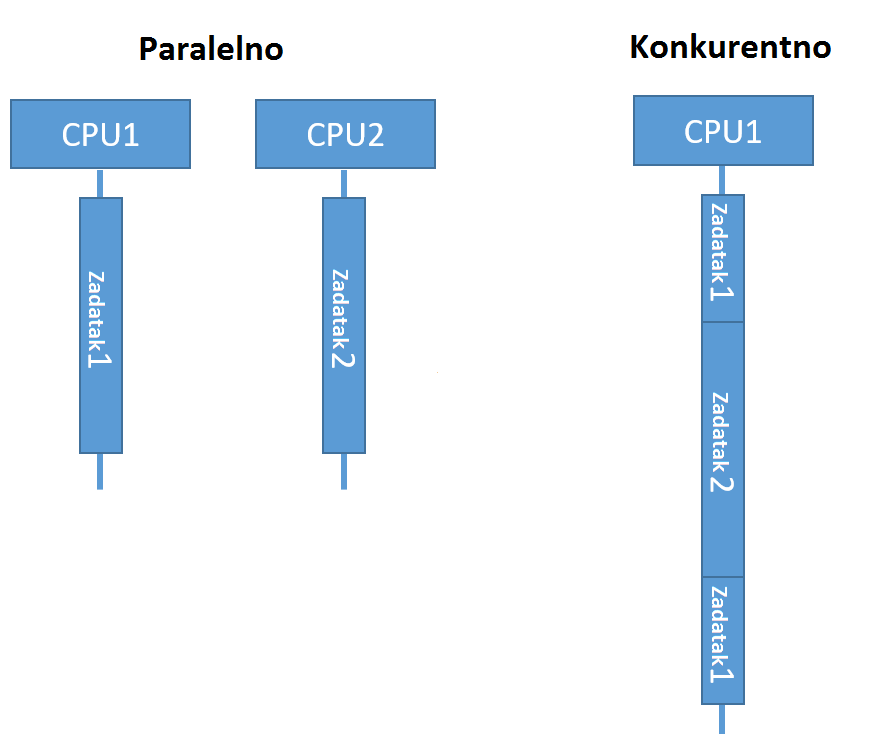
\includegraphics[width=0.6\textwidth]{parallel-vs-concurrent-dotnet-core.png}
%  \caption{Разлика између конкурентног и паралелног израчунавања}
%  \label{fig:ParVSCon1}
%\end{figure}
%
%\begin{figure}[!ht]
%  \centering
%  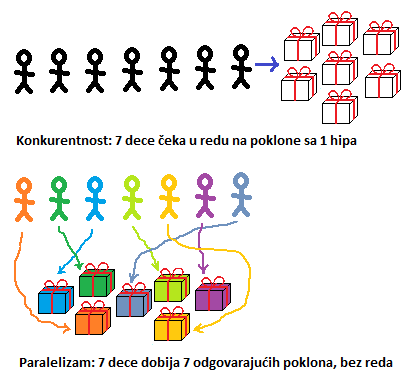
\includegraphics[width=0.6\textwidth]{parallelism-centric.png}
%  \caption{Разлика између конкурентног и паралелног израчунавања}
%  \label{fig:ParVSCon2}
%\end{figure}
%% Dve slike jedna pored druge
%%\begin{figure}[!tbp]
%%  \centering
%%  \subfloat[Flower one.]{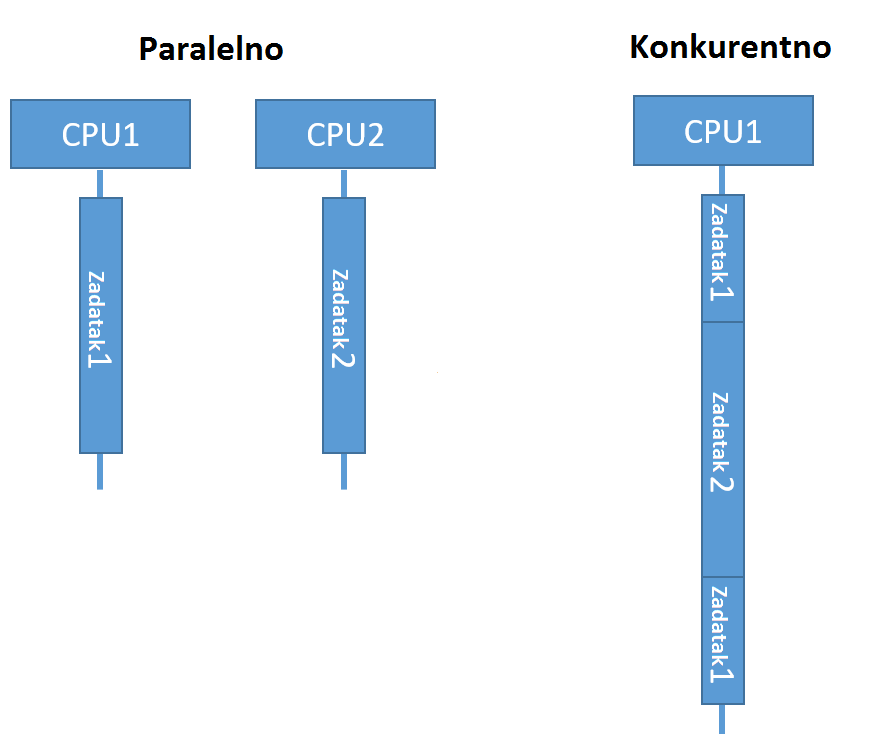
\includegraphics[width=0.5\textwidth]{parallel-vs-concurrent-dotnet-core.png}\label{fig:f1}}
%%  \hfill
%%  \subfloat[Flower two.]{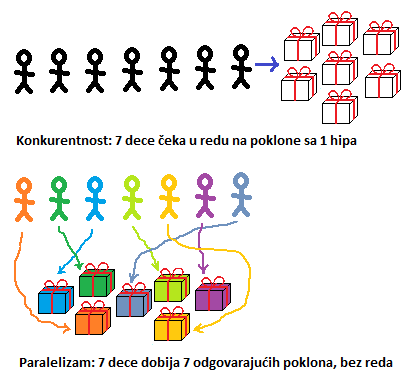
\includegraphics[width=0.5\textwidth]{parallelism-centric.png}\label{fig:f2}}
%%  \caption{My flowers.}
%%\end{figure}
%%
%---------------
\subsection{Модел дељења меморије}
Рад са нитима подржава модел дељења меморије (енг. \textit{shared memory model}). То значи да нити имају део меморије који им је заједнички, тако да могу асинхроно да приступају заједничким меморијским локацијама. То може довести до разних проблема. Ситуација када два или више процеса или нити истовремено читају и мењају исти податак се назива \textbf{надметање око ресурса} (енг. \textit{race conditions}). Један од тих процеса (или нити) поништи измене другог процеса, па резултат који се добије на крају зависи од редоследа којим се мења дати податак. Редослед је немогуће предвидети тако да се приликом покретања оваквог програма углавном сваки пут добије другачији резултат. Због оваквих проблема треба омогућити безбедно дељење ресурса, комуникацију и синхронизацију нити. Зато се прибегава техникама закључавања као што су мутекси, катанци, монитори, семафори. Сврха ових техника је спречити недозвољене приступе подацима који се деле. Некада је дозвољено истовремено читање података, а некада је строго забрањен приступ свим нитима осим оне која тренутно чита и/или мења податке. Такве одлуке се доносе у зависности од конкретног случаја и потреба \cite{progInScala3, survey}.

Механизми закључавања решавају проблеме који се тичу приступа подацима, али уводе нове проблеме \cite{progInScala3, microsoftRaceC}:
\begin{itemize}
\item \textbf{Број катанаца} Закључавање и откључавање катанаца представљају скупе операције. Због тога велики број катанаца може да успори рад програма. Са друге стране, мали број катанаца може значити да они закључавају велику количину података, што доводи до дужег чекања па и споријег рада. 
\item \textbf{Мртва петља} Мртва петља (енг. \textit{deadlock}) или \textit{узајамно закључавање} је ситуација када више процеса или нити уђе у стање чекања због тражења ресурса који није доступан. Све ове нити чекају да им нека друга ослободи ресурс, али је то немогуће јер нит коју чекају такође чека неки ресурс. Пример је дат на слици \ref{fig:deadlock}:
\begin{figure}[!ht]
  \centering
  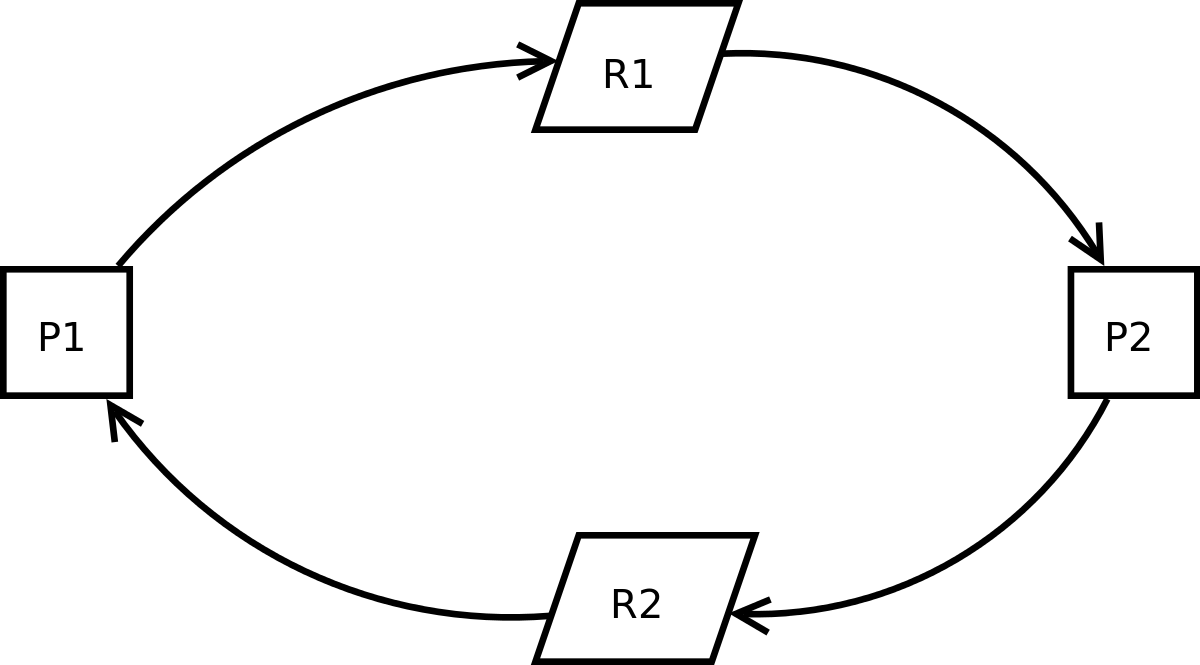
\includegraphics[width=0.5\textwidth]{deadlock.png}
  \caption{Мртва петља}
  \label{fig:deadlock}
\end{figure}
Процес P1 тражи ресурс R1 али не успева да му приступи јер процес P2 држи ресурс R1. Слично, процес P2 тражи ресурс R2 али њега држи процес P1. Два процеса су у застоју јер се међусобно чекају. Проблем мртве петље је последица лоше технике закључавања. Може се решити тражењем катанаца у унапред дефинисаном редоследу, али и даље представља оптерећење за програмере.

\label{raceCon}
\item \textbf{Тежак опоравак од грешака} Не постоји одређени механизам за опоравак програма са више нити од грешака. Углавном је корисно проћи кроз \textit{.log} датотеку у којој je у различитим тренуцима записанo стање стека са циљем праћења позивања функција и промена вредности променљивих.
\end{itemize}

Писање конкурентних програма је веома захтевно. Један од основних разлога што је ово захтеван посао је непредвидивост извршавања конкурентних програма. Немогуће је утврдити којим редоследом ће се послови обављати. Веома је компликовано доказати да је програм \textit{коректан} тј. да ради управо оно што се од њега очекује. Друга ствар која чини конкурентно програмирање захтевним је коришћење променљивих података. Дељени подаци који се временом мењају захтевају синхронизацију и механизме закључавања, отежавајући паралелизацију програма. То су разлози због којих је функционална парадигма погоднија од других за паралелизацију. Чим нема променљивих структура, нема ни проблема које оне носе са собом \cite{progInScala3}.

%---------------
\subsection{Модел размене порука}

Модел размене порука (енг. \textit{message passing model}) је један од популарних "трендова" који се тичу конкурентности. Овај модел подржава архитектуру \textbf{SN} тј. архитектуру \textit{Shared Nothing}. Архитектура \textit{SN} се односи на дистрибуиране системе и подразумева да се систем састоји из неколико независних чворова. Сваки чвор (тј. независна машина) има своју меморију, дискове и интерфејсе за улаз и излаз. Расположиви подаци се поделе овим чворовима тако да сваки од њих има одговорност искључиво за своје податке. Подаци се међу чворовима никада не деле, што значи да сваки чвор има потпуну слободу над својим делом посла. Због тога нема потребе за механизмима закључавања. Како се међу чворовима ништа не дели, отуда и назив ове архитектуре \cite{SNvsSD, warehouse}.

Оваква логика недељивости стоји и иза модела размене порука. Компоненте овог модела међусобно комуницирају искључиво размењујући поруке. Свака компонента овог модела има своје стање које јесте променљиво, али га никада не дели са другима. Поруке које се шаљу су \underline{непроменљиве} и могу се слати синхроно и асинхроно \cite{progInScala}.

Модел размене порука се може имплементирати на више начина, а најуспешнији начин је помоћу такозваног модела Актер (енг. \textit{Actors}). Њега је осмислио амерички научник Карл Еди Хјуит (енг. \textit{Carl Eddie Hewitt}) који је 1973. године заједно са другим ауторима објавио рад који представља увод у модел Актер. Иако се развија годинама, тек је од скоро доказано да је овај модел ефикасан у решавању проблема савремених рачунарских система. Он енкапсулира тежак рад са нитима и олакшава програмирање конкурентности. 

Компоненте модела Актер представљају објекти које зовемо \textit{Актери}. Они формирају хијерархијску структуру у којој сваки објекат има свог родитеља који сноси одговорност за њега. Сваки Актер има своје "поштанско сандуче" и његов задатак је да обради сваку поруку коју добије. Поруке се чувају у \textit{FIFO} (енг. \textit{first-in first-out}) структури тј. \textit{реду} (енг. \textit{queue}), па се поруке обрађују редом којим су стигле. Оно што разликује објекте Актер од других објеката је способност реаговања на поруке одређеном акцијом. Као одговор на поруку, Актер може направити још компонената Актер (своју децу), слати поруке другим компонентама или зауставити рад своје деце или себе. Актер има своје локално стање које је променљиво, али са другима не дели ништа осим порука. Важна особина Актерa је да се не блокирају када пошаљу поруку већ настављају са радом, односно слање порука је увек асинхроно. 

Предности модела Актер и уопште архитектуре \textit{SN} се огледају у избегавању свих поменутих проблема конкурентног програмирања, чији највећи узрок представљају дељени променљиви подаци. Модел Актер је погодан у апликацијама у којима је могуће посао поделити на што више мањих, независних послова. Тада сваки мањи посао представља задатак једне компоненте Актер. Родитељ решава проблеме своје деце и прикупља резултате њихових послова. Дизајн такве апликације личи на организацију послова у компанијама где се послови деле по одељењима, све док ти послови не постану довољно једноставни да их може обавити један радник. 

Иако модел Актер у многим случајевима олакшава посао, постоје ситуације када је неопходно да компоненте деле податке између себе. Не треба на силу користити један модел ако природа проблема намеће неки други. Модел Актер није универзално решење за све проблеме већ треба препознати случајеве када га није погодно користити. Неке од ситуација када треба прибећи другачијем решењу су следеће \cite{progInScala3}:

\begin{description}
\item \textbf{Дељени променљиви подаци} Неки проблеми природно захтевају дељење података. Тада је погодније изабрати директан рад са нитима и дељеном меморијом, поготово ако се подаци деле само за читање. Рад са базама података и трансакцијама је пример када се програмери обично одлучују за неко друго решење.
\item \textbf{Цена асинхроног програмирања} Модел дељења порука са собом носи одређену сложеност. Дебаговање и тестирање великих апликација које имплементирају модел дељења порука може бити веома тешко. Наиме, компликовано је праћење асинхроно послатих порука што доводи до тешког проналаска извора проблема. У овом случају је корисна информација о првој послатој поруци, тј. о поруци којом је започета комуникација међу компонентама. Такође, многим програмерима је тешко да се навикну на нову парадигму што изискује труд и време.
\item \textbf{Перформансе} Неке апликациjе захтеваjу наjвећу могућу брзину и ефикасност. Модел Актер енкапсулира рад са нитима чиме се налази на нивоу изнад њих. Боље перформансе програма се могу постићи директним радом са нитима уместо са моделом Актер.
\end{description}

Разни језици имају библиотеке које имплементирају модел Актер. У следећем поглављу је обрађена одговарајућа библиотека у Скали \cite{progInScala3, carlHewittActor, seven}.

% ------------------------------------------------------------------------------
\section{Библиотека \textit{Akka}}
\label{sec:akka}

\textbf{Akka} представља имплементацију модела Актер на Јава виртуелној машини. Од верзије 2.10 језика Скала ова библиотека је подразумевана библиотека за коришћење модела Актер. Постојала је и библиотека \textit{Actor}, али је она застарела и од верзије 2.11 се више не користи \cite{akkaMarius}.

Све што се тиче објеката Актер је смештено у способности \textit{Actor} које се уводи наредбом \textit{import}:
\begin{lstlisting}[language=Scala]
import akka.actor.Actor
\end{lstlisting}

Кључне особине које одликују компоненте Актер су слање и примање порука. То се ради на следећи начин \cite{progInScala3}: 
\begin{itemize}
\item Слање порука се врши позивом метода \textbf{!}:
\begin{lstlisting}[language=Scala]
a ! msg
\end{lstlisting}
Објекту \textit{a} се шаље порука \textit{msg}.
\item Примање порука се остварује помоћу блока \textbf{receive} и упаривања образаца које је објашњено у поглављу \ref{uparObr}:
\begin{lstlisting}[language=Scala]
receive {
	case pattern1 => 
		...
	case patternN => 
}
\end{lstlisting}
\end{itemize}

Све компоненте система Актер су хијерархијски распоређене и организоване тако да се свакој приступа на јасно дефинисан начин. То је описано у следећем поглављу.

\subsection{Структура}
\label{subsec:struktura}

Све компоненте Актер које припадају једној логичкој компоненти апликације (нпр. једна за управљање базом података а друга за реаговање на захтеве корисника) припадају заједничком систему који се назива \textbf{ActorSystem}. То је хијерархијски уређена група компоненти које деле исту конфигурацију. На \textit{ActorSystem} можемо гледати као на менаџера својих компоненти који прави нове и претражује постојеће компоненте. Такође, \textit{ActorSystem} је задужен за алоцирање нити које ће бити коришћене у апликацији \cite{progInScala3, akkaDoc}.

Све компоненте Актер једног система \textit{ActorSystem} су смештене у \textbf{стабло} које је приказано на слици \ref{fig:stablo}. Свака компонента има родитеља коме припада. На самом врху хијерархије налазе се три предефинисане компоненте \cite{akkaDoc}:
\begin{itemize}
\item компонента \textit{root guardian} је родитељ свих других компоненти. Чак и она интерно има свог родитеља који се назива \textit{Bubble-Walker}, али је он невидљив корисницима.
\item компонента \textit{user guardian} је родитељ свих корисничких компоненти (компоненти које су направили сами корисници) и сва њена деца испред свог назива имају префикс \textit{/user/}.
\item компонента \textit{system guardian} је родитељ свих интерних компоненти. Интерна компонента, на пример, може бити компонента коју направи сама конфигурација оног тренутка када се креира систем \textit{ActorSystem}. 
\end{itemize}

\begin{figure}[!ht]
  \centering
  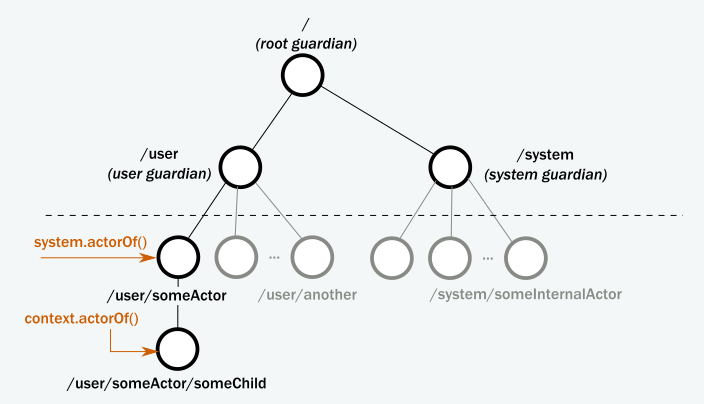
\includegraphics[width=1\textwidth]{akkaTree.png}
  \caption{Стабло компоненти Актер}
  \label{fig:stablo}
\end{figure}

Оваква хијерархијска структура је слична структури система датотека. Прву компоненту правимо помоћу метода \textit{actorOf} самог система \textit{ActorSystem}. Све компоненте направљене на овај начин ће постати деца предефинисане компоненте \textit{user guardian}. Овакве компоненте су на врху хијерархије корисничких компоненти, па за њих кажемо да су на највишем нивоу иако постоје предефинисане компоненте изнад њих. Компонента Актер која произведе нову компоненту представља њеног родитеља (енг. \textit{parent actor}), а нова компонента је њено дете (енг. \textit{child actor}). Ова радња се постиже методом \textit{actorOf} атрибута \textit{context} компоненте Актер. Овај атрибут је типа \textbf{ActorContext} који омогућава једној компоненти да има приступ самој себи, свом родитељу и својој деци. Свако дете добија име свог родитеља као префикс свог имена.

Прављењем компоненте Актер или добијањем постојеће претрагом система не добијамо директну референцу на компоненту, већ добијамо показивач на референцу \textbf{ActorRef}. Ова референца је задужена за слање порука својој компоненти и штити је од директног приступа корисника. Свака компонента има приступ својој референци преко атрибута \textit{self}. Слично, свака компонента преко атрибута \textit{sender} има приступ референци на компоненту која јој је послала поруку.

У систему \textit{ActorSystem} свака компонента Актер има путању \textbf{ActorPath} која је јединствено идентификује. Различите компоненте се могу налазити на различитим чворовима на мрежи тј. могу се извршавати на различитим Јава виртуелним машинама. Због тога први део путање садржи протокол и локацију на којој се налази компонента (идентификацију система \textit{ActorSystem} у коме се налази). Надаље путању чине надовезани елементи у стаблу раздвојени са "/", почевши од корена. На пример \cite{akkaDoc}:
\begin{lstlisting}[language=Scala]
"akka://my-sys/user/service-a/worker1"                  		   	 // lokalna komponenta
"akka.tcp://my-sys@host.example.com:5678/user/service-b" 	// udaljena komponenta
\end{lstlisting}
Код примера локалне путање протокол је "akka" a \textit{ActorSystem} je "my-sys". Међутим, нелокална путања дефинише другачији протокол и уз то име домаћина (енг. \textit{host}) и број порта. У обе путање присутне су поменуте компоненте "root guardian" и "user guardian" што чини део путање "/user". Након тога следе корисничке компоненте које добијамо проласком кроз стабло све до жељене компоненте.

Још једна сличност ове хијерархије са хијерархијом система датотека је начин на који претражујемо њене елементе. На пример \cite{akkaDoc}:
\begin{lstlisting}[language=Scala]
context.actorSelection("../*") ! msg
\end{lstlisting}
Метод \textbf{actorSelection} враћа референце компоненти које тражимо путем аргумента. Користећи "\textbf{..}" пењемо се један ниво изнад у стаблу тј. добијамо свог родитеља, а како "\textbf{*}" представља знак за било шта (енг. \textit{wildcard}), добијамо сву децу свог родитеља, укључујући и себе. На овај начин лако шаљемо поруку различитим компонентама истовремено.
%компоненту\footnote{Овде се не мисли на Actor компоненту као у остатку текста, већ на обичан елемент система ActorSystem.}
\par Сваки систем \textit{ActorSystem} има "диспечера" тј. елемент који се назива \textbf{MessageDispatcher}. Овај диспечер је задужен за слање порука у одговарајуће поштанско сандуче као и за позивање одговарајућег блока \textit{receive} компоненте Актер. У позадини диспечера налази се складиште нити која се назива \textit{thread pool}. Складиште садржи одређени број покренутих али неактивних нити које чекају да им се додели задатак. Сваки пут када је потребно извршити нови задатак, проверава се постојање слободне нити у групи. Ако постоји, бира се прва слободна нит. У случају да су све нити тренутно заузете, прва нит која се ослободи ће преузети нови задатак. Оваква идеја се примењује уколико знамо да ће бити пуно нити које ће извршавати кратке задатке, па је ефикасније имати унапред спремне нити него их изнова и изнова правити. На овај начин се такође смањује број нити које се креирају током рада апликације.

\textit{Thread pool} даје важну гаранцију у конкурентној апликацији, а то је да у сваком тренутку само једна нит може извршавати одређену компоненту Актер. То значи да никада две или више нити не могу истовремено извршавати исту компоненту. Једну компоненту могу извршавати различите нити али само у различитим временским интервалима. То нам омогућава да безбедно мењамо податке унутар компоненте Актер докле год те податке не делимо \cite{progInScala3, akkaDoc}. 
\par Компонента која је задужена за примање порука које су послате обустављеној или непостојећој компоненти назива се \textit{dead letter actor}, а њено сандуче \textit{dead letter mailbox}. Након што се одређена компонента угаси, није добра пракса направити нову са истом путањом. Разлог томе је то што не можемо претпоставити редослед догађаја и може се десити да нова компонента прими поруку која је била намењена старој \cite{akkaDoc}.
\par Један од разлога због којих су компоненте смештене у хијерархијску структуру је управљање њиховим животним циклусима. Компоненте живе до момента када их корисник заустави и тада се прво рекурзивно заустављају сва њена деца. Ниједно дете не може надживети свог родитеља. То је корисно јер се на тај начин спречава цурење ресурса. Такође, препоручује се заустављање компоненте једино из ње саме. Добра је пракса да компонента као одговор на одређену поруку заустави саму себе, док се заустављање произвољне компоненте из неке друге избегава.

Други разлог постојања хијерархије је управљање грешкама и изузецима. \textit{Akka} подржава програмирање у коме се стање грешке посматра као било које друго валидно стање. Немогуће је спречити све грешке, тако да је циљ припремити начине на које ћемо се изборити са њима. У томе помаже структура компонената. Када компонента наиђе на проблем она привремено суспендује сву своју децу и саму себе, и обавештава родитеља о проблему. Њен родитељ одлучује како даље наставити са радом. Другим речима, сваки родитељ је задужен за решавање грешака и изузетака своје деце и тиме представља њиховог \textit{супервизора}. Акција коју родитељ одлучи да предузме назива се \textit{стратегија супервизора} (енг. \textit{supervisor strategy}). Подразумевана стратегија је заустављање и поново покретање (рестартовање) детета, које подразумева брисање акумулираног стања и враћање на почетак. Ову акцију је могуће предефинисати, тако да поред рестартовања постоје још три опције које родитељ може предузети \cite{progInScala3, akkaDoc}:
\begin{enumerate}[1)]
\item Настављање са радом са акумулираним стањем
\item Трајно заустављање детета
\item Пропагирање грешке на ниво изнад тј. обавештавање свог родитеља о њој и тиме суспендовање себе
\end{enumerate}

Што се тиче самог рестартовања, разликујемо две стратегије: \textit{One-for-One} и \textit{All-for-one}. Ове стратегије говоре о томе шта се дешава са осталом децом супервизора тј. родитеља компоненте која се рестартује. Стратегије су илустроване на сликама \ref{fig:oneForOne} и \ref{fig:allForOne} \cite{progInScala3, akkaDoc}:
\begin{itemize}
\item \textbf{One-for-One} је подразумевана стратегија у којој током рестартовања одређене компоненте, друге компоненте истог родитеља живе и настављају са радом независно од ње. Ова стратегија се примењује када компонента врши посао који не утиче на послове других компоненти.
\item \textbf{All-for-One} стратегија се примењује када компоненте заједно учествују у неком послу тако да рестартовање једне повлачи рестартовање и осталих компоненти. У овом случају рестартовање једино компоненте у којој се јавила грешка не би било валидно.
\end{itemize}

\begin{figure}[!tbp]
  \centering
  \subfloat[One-for-One]{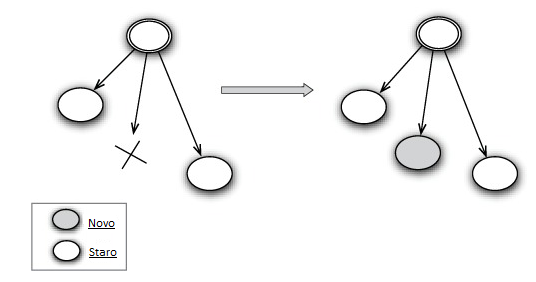
\includegraphics[width=0.5\textwidth]{oneForOne.png}\label{fig:oneForOne}}
  \hfill
  \subfloat[All-for-One]{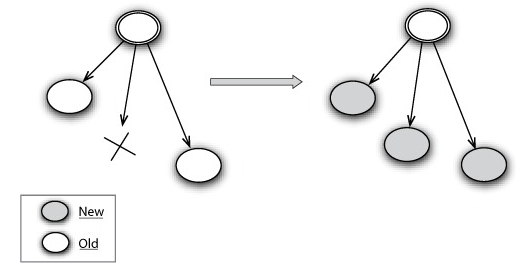
\includegraphics[width=0.5\textwidth]{allForOne.png}\label{fig:allForOne}}
  \caption{Стратегије рестартовања}
\end{figure}

%\subsection{Future и Promise објекти}
%\label{subsec:futPro}

%--------

% ------------------------------------------------------------------------------
\chapter{Расплинуто тестирање}
\label{chp:rasplTestiranje}

Грешке су саставни део сваког посла. Развојем софтвера развијају се нове врсте пропуста. "Постоје стотине слабости софтвера које само чекају да буду откривене, и биће откривене када прође довољно времена" \cite{fuzzing}. Неке грешке немају велики значај, док друге могу оставити озбиљне последице. Постоје програми који користе грешке других програма уметањем вируса, црва, злонамерних скриптова и слично. Циљ напада на софтвер може бити преузимање или пад система, крађа, злоупотреба и мењање постојећих података, производња нових и лажних података итд.  Зато је јако важно софтвер тестирати са циљем елиминисања што већег броја грешака које могу угрозити квалитет и безбедност система \cite{fuzzing, bezbMalkov}.

Тестирање се може применити на разне аспекте система, због чега постоје различите врсте тестова. На пример, неким тестовима је циљ провера тачности израчунавања вредности израза или функције. Другачијом врстом тестова можемо проверити на који начин независне јединице система раде једна са другом, итд. Због тога је важно напоменути да је у овом раду фокус на тестирању робусности софтвера. Циљ тестирања је откривање неисправног или непредвидивог понашања програма у случају неисправних улазних података. 

Расплинуто тестирање (енг. \textit{fuzz testing/fuzzing}) је приступ тестирању софтвера који се бави генерисањем великог броја улаза у програм, након чега за сваки од улаза посматра његов ток извршавања. Циљ ових тестова је да открију необичне грешке и изузетке у програму. Улази треба да буду неочекивани и генеришу се или потпуно случајно или уз коришћење одређених \textit{хеуристика}. Узимају се у обзир и неисправни улази јер је важно да програм препозна и одбаци овакве улазе без прекида или отежавања даљег рада. %"Расплинуто тестирање на своју мету баца све осим кухињске судопере и посматра резултате" %\cite{fuzzingBrute}. 

\section{Основе тестирања софтвера}
\label{sec:osnoveTestiranja}

Тестирање софтвера представља најчешћи вид верификације софтвера. \textit{Верификација} софтвера се бави испитивањем исправности програма тј. провером жељеног понашања програма задатог \textit{спецификацијом}. Постоје \textit{статичка} и \textit{динамичка} верификација. Статичка испитује исправност програма без извршавања кода тј. његовом анализом, док динамичка подразумева испитивање извршавањем кода \cite{milenaDokt}. 

Тестирање се може описати на више начина. Често се описује као процес коме је циљ процена квалитета софтвера. Овакву дефиницију тестирања треба узети са резервом. Тестирање нам свакако даје увид у квалитет софтвера али прилично мали, јер углавном случајеви које тестирамо представљају само кап у океану свих могућих случајева. Мање амбициозна дефиниција представља тестирање као процес који покушава да открије грешке у програму посматрајући његово извршавање у контролисаним условима \cite{testPrinc}.

Технике тестирања софтвера константно напредују, али треба имати у виду њихова ограничења. Холандски информатичар и добитник Тјурингове награде Едсхер Даикстра (хол. \textit{Edsger Wybe Dijkstra}) је рекао: "Тестирање софтвера може показати присуство грешака, али никада њихово одсуство" \cite{testPrinc}. Тестирање не може доказати исправност софтвера, већ се за то користе друге, математичке технике. Ипак, тестирање има важну улогу у свим фазама развоја софтвера. Помоћу њега смањујемо број промаклих грешака и повећавамо поузданост изграђеног система.

Због ефикасности процеса тестирања, често је пожељна његова аутоматизација. Генерисање тест примера је у већини случајева потребно извршити ручно, мада постоје неке врсте тестирања у којима је могуће аутоматизовати овај процес. Што се тиче извршавања тест примера, аутоматизација је углавном могућа и њу подржавају разни алати за развој софтвера.

Важно је на који начин се приступа тестирању софтвера. Некада је дизајн тестова једнако компликован као дизајн самог програма. Било да се тестирање врши ручно или аутоматизовано, пожељно је имати планове и идеје о тест примерима који су вероватнији да изазову грешку од других. Треба одредити и редослед којим ће се извршавати осмишљени тестови. Редослед је важан јер постоје случајеви када се одређени тест примери не могу извршити пре извршавања неке друге радње. Рецимо, не можемо тестирати брисање податка из базе података ако је она празна тј. ако претходно није успео тест уметања податка у базу. Након извршавања тестова прегледају се добијени резултати и утврђује се спремност тестираног система. Сав посао везан за тестирање може вршити сам програмер који је уједно и тестер. Друга могућност је постојање тестера који поред програмирања разуме технике тестирања, познаје грешке које се често јављају и необичне случајеве који их производе. Он може али не мора да ради у договору са програмером \cite{guideTestDesign, testMilena}.

"Покривеност кода (енг. \textit{code coverage}) тестовима је однос броја неких елемената програма испитаних тестовима у односу на укупан број тих елемената" \cite{testMilena}. Уопштено, покривеност представља неку врсту метрике која говори о броју случајева који су испитани тестовима. Када сматрамо да тестови испитују добар део програма, кажемо да тестови "покривају" велики број случајева тј. да имају висок ниво покривености. У зависности од изабраних елемената програма разликујемо покривеност путања, наредби, грана/одлука, услова, вишеструких услова и функција. Постоје различити алати за рачунање нивоа покривености кода \cite{testMilena}.
%-------------
\subsection{Нивои тестирања}
\label{subsec:nivoiTest}

\par Тестирање се врши на више нивоа, у зависности од сложености компонената које се тестирају. Почиње се од \textbf{тестирања јединица кода} (енг. \textit{unit testing}), тј. независних делова система. Јединице представљају најмање независне целине које обављају неку функцију (нпр. класа или функција). Пре спајања више независних јединица, важно је да оне саме раде правилно, изоловане од других јединица. Други ниво, \textbf{компонентно тестирање} (енг. \textit{component testing}), је веома слично првом нивоу. Компоненте су изоловане од других компонената, али су мало веће и јединице које су у њима нису изоловане једне од других. Трећи ниво је \textbf{интеграционо тестирање} (енг. \textit{integration testing}). Оно је задужено за тестирање компоненти које заједно чине целину система. То је важно јер се неретко дешава да компоненте које савршено раде самостално не успевају добро да раде заједно и да комуницирају једне са другима. Следећи ниво тестира систем као целину и зато се назива \textbf{системско тестирање} (енг. \textit{system testing}). На овом нивоу се тестира и хардвер, а тестирање не обухвата само функционалност програма већ и безбедност, капацитет, перформансе, преносивост, итд. На овом нивоу се примењује \textbf{истраживачко тестирање} (енг. \textit{exploratory testing}) током кога тестер извршава тест случајеве који нису били у плану, са намером да открије непредвиђене начине коришћења система. Обављају се и \textbf{тестови прихватљивости} (енг. \textit{acceptance testing}) које извршавају корисници, проверавајући да ли софтвер испуњава њихова очекивања и потребе. Након измена система врши се \textbf{регресионо тестирање} (енг. \textit{regression testing}) које треба да покаже правилан рад неизмењених  функција. Такође треба да покаже и да су перформансе новог система макар једнаке перформансама старог система, а пожељно је да су боље. Сви ови нивои се примењују уколико време дозвољава темељно тестирање. У случају мањка времена, тестирање се прилагођава могућностима \cite{guideTestDesign, testMilena}.

%-------------
\subsection{Стратегије тестирања}
\label{subsec:stratTest}

На основу доступних информација о имплементацији софтвера који се тестира разликујемо три основне стратегије тестирања \cite{fuzzingBrute, fuzzing, testMilena}: 

\begin{description}
\item \textbf{Тестирање беле кутије} (енг. \textit{white box testing}) или \textit{структурно} (енг. \textit{structural testing}) тестирање подразумева познавање интерне структуре и имплементације програма. Тестерима је доступан целокупан изворни к\^{о}д, тако да је њихов посао да га детаљно изуче како би нашли делове који су подложни грешкама. То је мукотрпан посао јер подразумева пролажење кроз све линије кода којих често има превише за људску обраду. Због тога се углавном користе алати који скенирају к\^{о}д и региструју потенцијалне слабости програма. Након тога их проверава програмер и одлучује да ли су пронађене слабости заиста претња. Алати много помажу али не могу да замене знање и искуство стручњака. 
\par Добра страна ове стратегије је што доступност изворног кода омогућава високу покривеност кода (можемо проћи кроз велики број путања кроз програм, кроз много грана, итд.). Ипак, велики број линија кода повлачи и велику сложеност његовог анализирања. Алати који анализирају к\^{о}д често окарактеришу пуно делова кода као потенцијалне слабости. Тада програмери морају проћи кроз дугачак извештај о њима, а углавном се испостави да је већина записаних слабости лажна узбуна. Такође, ова стратегија је непримењива уколико изворни к\^{о}д није доступан. Треба имати у виду да је доступност кода уобичајена код програма на \textit{Linux} оперативним системима, што није случај код програма писаних за \textit{Windows} оперативне системе. 

\item \textbf{Тестирање црне кутије} (енг. \textit{black box testing}) или \textit{функционално} (енг. \textit{functional testing}) не користи никакве информације о интерној структури и имплементацији програма. Ова стратегија се може применити када информације о унутрашњој структури нису доступне, али је корисна и када јесу доступне, поред тестирања беле кутије. Једине информације које се користе су улаз и излаз из програма. Тестирање се углавном заснива на претпоставкама о тестираном програму, његовим спецификацијама и налажењу прихватљивог броја репрезентативних тест примера.
\par Једна од предности ове стратегије је примењивост. Без обзира на доступне информације, тестирање црне кутије је најчешће могуће и најчешће једноставније од других врста тестирања. Погодно је јер га могу примењивати и тестери који нису програмери. Такође, због тога што се тестови не ослањају на унутрашњу структуру софтвера, исти тест можемо употребљавати више пута за различите програме сличне намене. Једноставност овог приступа има и своје мане. Пошто се тестирање врши на основу претпоставки, никада не можемо тачно проценити ефикасност тестирања и ниво покривености кода као код тестирања беле кутије. Такође, ова стратегија није погодна за комплексне нападе где је потребно извршавати тестове одређеним редоследом ради изазивања рањивог стања програма.

\item \textbf{Тестирање сиве кутије} (енг. \textit{gray box testing}) представља комбинацију претходне две стратегије. Једна могућност је да се тестови базирају на обема техникама беле и црне кутије. Друга могућност је да у некој мери постоје информације о унутрашњој структури софтвера, али не као код тестирања беле кутије. Изворни к\^{о}д није доступан али се увид у структуру софтвера добија преко датотека компајлираног програма тј. његових бинарних извршних датотека. Како су ове датотеке нечитљиве за људе, на њих се примењује процес обрнутог инжењеринга (енг. \textit{reverse engineering}). Обрнути инжењеринг не може да открије изворни к\^{о}д програма, али препознавањем одређених инструкција може да произведе формат који се налази између изворног кода и машинског кода. За разлику од бинарних датотека, овај формат је читљив за људе и омогућава анализу сличну као код структурног тестирања. 
\par Тестирање сиве кутије је хибридно решење које може искористити предности стратегија црне и беле кутије. Уколико изворни к\^{о}д није доступан а бинарне датотеке јесу, често се користи обрнути инжењеринг као допуна чистом тестирању црне кутије. Мана ове стратегије је велика сложеност обрнутог инжењеринга који захтева постојање богатих ресурса.
\end{description}

Свака од поменутих стратегија има своје предности и мане. Ни за једну се не може рећи да је генерално боља од других, јер је свака од њих погодна за откривање различитих врста слабости. Најбоље решење је применити више стратегија ради откривања што више грешака. Различитост стратегија илустрована је сликом \ref{fig:boxes}.

\begin{figure}[!ht]
\centering
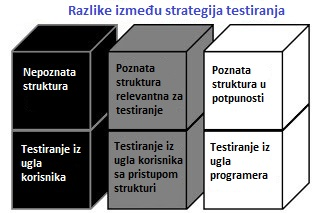
\includegraphics[width=0.5\textwidth]{boxes.jpg}
\caption{Разлике између стратегија тестирања}
\label{fig:boxes}
\end{figure}
% (енг. \textit{})

\section{Основе расплинутог тестирања}
\label{sec:osnoveRasplTestiranja}

Развојем расплинутог тестирања је откривено доста начина генерисања улаза који у великом броју случајева откривају грешке. Најчешће се улази или делови улаза генеришу случајно, праве се улази који су мањи него што би требало (нпр. датотека са мање података), користе се негативне и граничне вредности нумеричких типова података, предугачке ниске карактера, ниске карактера са специјалним карактерима, замењују се суседни битови, итд. Не постоје правила која дефинишу радње које се примењују на подацима, већ само савети до којих се дошло дугогодишњим испробавањем.

Савети који помажу при генерисању тест примера представљају \textit{хеуристике}. Хеуристика је приступ решавању проблема који прави изборе на основу искуства, тј. изборе који ће највероватније довести до решења проблема. То су избори за које не постоји доказ да доводе до решења, али се у пракси показало да дају добре резултате. Хеуристике се користе у случају да је немогуће или је јако тешко испитати све могуће случајеве неког проблема. Зато се испитају познати случајеви који углавном у кратком временском периоду нађу решење. Решење често не буде најбоље могуће решење, али буде прихватљиво \cite{heuristics}.

Кључна предност расплинутог тестирања наспрам других техника тестирања је могућност аутоматизације овог процеса. Ручно креирање тест примера и покретање програма је веома напорно, споро, неефикасно и захтева да га обавља стручњак у области тестирања. Зато се прибегава аутоматизацији што је могуће већег дела посла које тестирање захтева. Тестирање може покренути особа без великог знања о томе. Такође, многе апликације за тестирање су примењиве на велики број различитих програма \cite{fuzzingBrute, fuzzing}.

Расплинуто тестирање је један од приступа тестирања црне кутије. Програм за тестирање не зна ништа о структури програма који тестира. Проблем који се јавља оваквим тестирањем је тај што формирани улази често откривају грешке које је лако открити. То су грешке до којих долази извршавањем кода који се најчешће извршава. Са друге стране, семантичке грешке које се налазе дубоко у програму остају неоткривене. Зато су развијени приступи алтернативног расплинутог тестирања који одговарају тестирању црне, беле и сиве кутије \cite{fuzzing, grayBoxFuzzing, whiteBoxFuzzing}:
\begin{description}
\item\textbf{Расплинуто тестирање црне кутије} (енг. \textit{black box fuzzing}) је приступ на који се обично мисли под појмом "расплинуто тестирање". Он је најлакши за имплементацију и омогућава тестирање великог броја тест примера за кратко време. Показује се да је често ефикаснији од других приступа уколико њима треба превише времена за генерисање тест примера.
\item\textbf{Расплинуто тестирање беле кутије} (енг. \textit{white box fuzzing}) пре самог тестирања користи технике које идентификују делове програма који могу да имају грешке. На тај начин ова врста тестирања повећава покривеност кода, открива грешке до којих се теже долази него другим врстама тестирања, али је и компликованија од њих. 
\item\textbf{Расплинуто тестирање сиве кутије} (енг. \textit{gray box fuzzing}) је приступ који има предности претходне две технике а труди се да избегне њихове мане. Тежи се да ефикасност буде што ближа ефикасности приступа црне кутије, али ова техника не генерише улазе "на слепо" већ користи неки паметнији начин, као приступ беле кутије. Уместо анализе кода, користe се технике инструментације да се добије увид у структуру програма.
\end{description}

\subsection{Историја}
\label{subsec:history}

Примена тестирања налик на расплинуто је почело још 1980-их година са алатом званим "мајмун" (енг. \textit{Тhe monkey}). Он је развијен за тестирање програма на \textit{Macintosh} рачунарима, који су имали проблема због мањка меморије. Мајмун је симулирао правог мајмуна који неартикулисано удара у тастатуру и миш рачунара и на тај начин тестира рад покренутог програма. Ипак, до 1990-их су интересовања и потребе за тестирањем биле много мање него данас, највише због недостатка интернета и идеја напада на други софтвер. Истраживање безбедности софтвера је почело крајем 1980-их година, када су почели да се развијају напади који се односе на прекорачење бафера. Један од познатих напада је настао 1988. године и назива се "Morris Internet Worm" \cite{fuzzingBrute, fuzzing}. 

Први пројекат развијен за тестирање је написан 1989. године. Идеју за овај пројекат је добио професор Бартон Милер (енг. \textit{Barton Miller}), за кога неки сматрају да је "отац" расплинутог тестирања. Заједно са својим ученицима са курса о оперативним системима тестирао је квалитет и поузданост \textit{UNIX} апликација. Програм је случајно генерисао ниске карактера и прослеђивао их апликацијама. Иако је тестирање имало веома једноставну идеју, у то време је то био велики помак јер се о расплинутом тестирању знало јако мало. На Универзитету у Оулу у Финској је 1999. године почело развијање пакета тестова под називом \textit{PROTOS}. Ови тестови су проверавали безбедност разних протокола. Компанија \textit{Microsoft} је 2002. године новчано помогла овој иницијативи тако да је тим који је развијао \textit{PROTOS} 2003. године засновао компанију за производњу пакета тестова, под именом \textit{Codenomicon}. Након тога, објављен је програм за тестирање отвореног кода имена \textit{SPIKE}. Он је био напреднији од програма који је развио професор Милер. Брзо је почело и развијање других пројеката попут \textit{sharefuzz}, \textit{mangleme}, \textit{Hamachi}, \textit{CSSDIE}, \textit{FileFuzz}, \textit{SPIKEfile}, \textit{notSPIKEfile}, итд. Компанија \textit{Mu Security} je 2005. године почела да развија хардверски уређај коме је циљ мењање података који се шаљу протоколима путем мреже. Контроле \textit{ActiveX} су такође постале мета програма \textit{COMRaider} и \textit{AxMan} 2006. године \cite{fuzzingBrute, fuzzing}. Временом је потреба за сигурношћу софтвера постајала све већа, тако да су се развијали алати за најразличитије врсте апликација. Методе тестирања, као и апликације које врше тестирање, се и данас развијају и побољшавају. Доступан је велики број алата који примењују најновије технике тестирања и врше разне оптимизације ради веће ефикасности. Оптимизације омогућавају краће време и цену тестирања, једноставност коришћења, минималну људску интеракцију, итд. Неки од алата имају специфичну примену, док су други употребљиви у свакој врсти софтвера. Неки од познатијих алата су \textit{AFL}, \textit{Project Springfield}, \textit{OSS-Fuzz}, \textit{libFuzz}, \textit{BFuzz}, \textit{Fuddly}, \textit{Honggfuzz}, \textit{Peach}, \textit{Radamsa}, итд \cite{bestFuzzers, fuzzingBrute, fuzzing}. 

\subsection{Ограничења}
\label{subsec:ogranicenja}

Различите врсте тестирања откривају различите врсте слабости. Не постоји универзална техника за откривање свих грешака, већ у зависности од потреба бирамо одређену технику. Неке од врста проблема које расплинуто тестирање обично не открива су \cite{fuzzingBrute}:
\begin{description}
\item \textbf{Права приступа} Неки програми разликују обичне од привилегованих корисника који имају више права од обичних (рецимо поред читања података могу да их бришу или мењају). Програм за расплинуто тестирање не зна ништа о логици програма који тестира, због чега не разликује типове корисника. Извршавање недозвољених функција од стране обичног корисника ће проћи неопажено код програма за расплинуто тестирање. Могуће је уметнути логику програма у програм за тестирање, али је то веома сложен процес.  
\item \textbf{Дизајн програма} Неки програми имају мане које се односе само на јако лоше осмишљен дизајн. Пример је апликација која дозвољава свим корисницима приступ одређеним подацима. Велика је грешка не узимање у обзир злонамерне кориснике. Проблем је непостојање аутентикације и ауторизације. Програм за расплинуто тестирање не може да препозна овакав безбедносни проблем.
%\item \textbf{Задња врата} ????????
\item \textbf{Безбедност меморије} Једна од врста напада на софтвер може бити приступање недозвољеној меморији. Читањем и писањем на разне меморијске локације нападач може да стекне одређену контролу над програмом. Недозвољен приступ меморији може да се препозна на нивоу инструкције машинског кода, након чега се програму пошаље сигнал \textit{SIGSEGV}. Проблем је у томе што неретко програми сами решавају овај проблем тако што "ухвате" сигнал и реагују одређеном акцијом. Реаговање на погрешан начин може бити опасно, као нпр. игнорисање сигнала. Програм за расплинуто тестирање често не примети овакву врсту слабости јер је она решена (правилно или неправилно) од стране самог програма.
\item \textbf{Сложени напади} Расплинуто тестирање је корисно за детекцију индивидуалних слабости. Међутим, није се добро показало у случају сложених напада који искоришћавају више слабости истовремено.
\end{description}

\section{Врсте програма расплинутог тестирања}
\label{sec:vrsteProRaspTest}

Програми расплинутог тестирања се разликују по разним карактеристикама. Две основне поделе ових програма се односе на начин на који генеришу тест примере и на тип самог програма који тестирају.

Начин генерисања тест примера има два основна критеријума.
Први критеријум представља постојање почетних тест примера од којих се генеришу нови тест примери \cite{fuzzingBrute, fuzzing}:
\begin{itemize}
\item \textbf{Тестери засновани на мутацијама} (енг. \textit{mutation-based fuzzers}) користе постојеће тест примере за генерисање нових, примењујући измене тј. мутације на улазним подацима. Квалитет тестирања зависи од квалитета постојећих тест примера. Ови тестери су обично тестери опште намене. 
\item \textbf{Тестери засновани на генерацијама} (енг. \textit{generation-based fuzzers}) генеришу тест примере "од нуле" тј. независно од постојећих. Једине информације које могу да користе су информације о формату који тест примери треба да задовоље (нпр. формат датотека или одређени протокол). Обично су овакви тестери специфични за одређени проблем.
\end{itemize}

Програми за расплинуто тестирање, независно од тога да ли су засновани на мутацијама или генерацијама, у некој мери користе случајне податке за генерисање тест примера. Могуће је све податке генерисати случајно, што доводи до тежег увиђања тачног низа догађаја који је довео до грешке. Друга могућност је да се на основу спецификације програма креирају тест примери који ће тестирати граничне вредности података, које су често критичне. Најбоље резултате даје генерисање тест примера комбинацијом ове две технике.

Мутацијски и генерацијски тестери су основни типови тестера. Поред њих постоји још један тип тестера који се заснива на напредној техници која се назива \textbf{еволуционо расплинуто тестирање} (енг. \textit{evolutionary fuzzing}). Ова техника се заснива на "учењу". На основу претходних корака, тестер закључује које тест примере би требало даље да конструише. Рецимо, за сваки тест пример тестер може да процени покривеност кода, и закључи на који начин да измени тест пример тако да покривеност буде већа. Еволуционо тестирање се ослања на друге технике, попут техника генетских алгоритама \cite{fuzzing, 15minuteGuide}.

Други критеријум који дели програме за тестирање на основу начина генерисања тест примера је присуство или одсуство знања о томе како треба да изгледају улази у програм који се тестира \cite{fuzzingBrute, fuzzing}:
\begin{itemize}
\item \textbf{Интелигентни тестери} (енг. \textit{intelligent fuzzers}) познају структуру улазних података програма који се тестира. На тај начин се избегава генерисање података које би програм одбацио пре било каквог рада над њима. Имплементација интелигентног тестера је компликована јер захтева проучавање структуре података који представљају улазе у програм.
\item \textbf{Неинтелигентни тестери} (енг. \textit{non-intelligent}/\textit{dumb fuzzers}) конструишу улазне податке за програм "на слепо" тј. не знајући ништа о структури тих података. На тај начин тестер може генерисати велики број улаза који ће брзо бити одбачени од стране програма.
Њихова имплементација је једноставнија од имплементације интелигентних тестера.
\end{itemize}

Ако улаз у програм представља датотека одређеног формата, неинтелигентни тестер може да генерише тест примере тако што инвертује произвољне битове те датотеке. Са друге стране, интелигентни тестер намерно оставља неке делове датотеке неизмењеним а друге делове мења. Рецимо, ако структуру чине називи поља и њихове вредности, називи ће остати исти док ће се вредности мењати.

Интелигентни тестери углавном имају већу покривеност кода и могу да укажу на већи број грешака од неинтелигентних, али то није правило. Најбоље је креирати тестер који не иде ни у једну крајност, јер то води до лоших резултата. Тестер који не зна ништа о формату улаза може да креира бескорисне тест примере, али може и да пронађе неочекивану слабост система да се носи са неисправним улазима. Са друге стране, интелигентни тестер избегава губљење времена непотребним тест примерима, али обично претпоставља исправан рад неких функција система. Неретко се деси да овакав тестер не ради добро јер прави исте претпоставке које је правио и програмер који је писао програм, због којих и долази до одређених грешака. Такође, интелигентни тестер може бити превише скуп због своје сложености. Балансиран приступ је најбоље решење: направити тестер који је довољно интелигентан да смањи време извршавања програма, али да не буде превише сложен и скуп, као и да не ослаби способност тестирања.
%%%%%%%

Неки аутори поистовећују тестере засноване на мутацијама са неинтелигентним тестерима, а тестере засноване на генерацијама са интелигентним тестерима. Такво поистовећивање није исправно. Тестери засновани на мутацијама најчешће заиста јесу неинтелигентни јер обично не узимају структуру улаза у обзир 
већ мењају битове постојећих улаза. Ипак, то није правило. Постоје и интелигентни тестери засновани на мутацијама који парсирају постојеће улазе да не би креирали оне које би програм одмах одбацио.
Слично, тестери засновани на генерацијама могу бити неинтелигентни, иако је то веома редак случај. Рецимо, тестер који генерише улазе случајним подацима, без постојећих улаза, технички спада у тестере засноване на генерацијама. 

% ******************************

У зависности од природе програма који се тестира, тестер који врши тестирање тог програма се може сврстати у неку од следећих категорија \cite{fuzzingBrute, fuzzing}:
\begin{description}
\item \textbf{Локални тестери} (енг. \textit{local fuzzers}) У ову категорију се сврставају тестери разних локалних програма. Класичан пример програма који су погодни за расплинуто тестирање су програми који омогућавају обичном кориснику да привремено (за време његовог извршавања) добије одређене привилегије. На \textit{Unix} системима има неколико таквих подразумеваних апликација (енг. \textit{setuid applications}), а то се може подесити и за друге. Слабости у оваквим програмима представљају велику опасност јер би грешкe моглe да омогућe кориснику да трајно добије привилегије и извршава произвољан к\^{о}д. Расплинуто тестирање проналази слабости ових апликација тако што их покреће са трансформисаним аргументима. Аргументи се могу слати програму у виду аргумената командне линије (енг. \textit{command-line fuzzers}), у виду променљивих окружења (енг. \textit{environment variable fuzzers}), или у виду датотека одређеног формата (енг. \textit{file format fuzzers}).
\item \textbf{Тестери удаљених програма} (енг. \textit{remote fuzzers}) Ови тестери тестирају програме који се извршавају на удаљеним чворовима. Међу њима постоје две врсте тестера. 

Прву врсту чине тестери мрежних протокола (енг. \textit{network protocol fuzzers}). Тестирају се једноставни и сложени протоколи. Једноставни су они који имају слабу аутентикацију или је уопште немају, користе \textit{ASCII} карактере уместо бинарних података, итд. Сложени протоколи се састоје углавном из бинарних података међу којима се налази понекa \textit{ASCII} ниска карактера. Аутентикација је сложенија и често се за проверу послатих података користе дужина или збир података.  

Другу врсту чине тестери Веб апликација (енг. \textit{Web application fuzzers}). Они комуницирају помоћу \textit{HTTP} протокола. Веома су важни јер данас имамо јако много апликација на Вебу с којима су се развиле и слабости јединствене за њих попут уметања \textit{SQL} упита (енг. \textit{SQL injection}), уметање скриптова (енг. \textit{cross site scripting}), онемогућавања услуге (енг. \textit{denial of service}) и многих других.

\item \textbf{Меморијски тестери} (енг. \textit{in-memory fuzzers}) Ови тестери су корисни када су неке друге врсте неефикасне. Њихове идеје су једноставне и заснивају се на измени аргумената функција програма директно у меморији, при чему се мењају и аргументи који иначе нису доступни кориснику. Имплементације оваквих тестера су веома компликоване. Постоји више приступа оваквом тестирању. Један приступ подразумева замрзавање процеса и чувања његовог тренутног стања које се касније поново користи тј. изазове се без поновног покретања процеса. Након тога, у свакој итерацији се у процес у таквом стању уметну неисправни улазни подаци, посматра се резултат и враћа се на сачувано стање. На овај начин се добија на брзини и ефикасности јер се делови програма који су неважни за тестирање прескачу (замрзавањем стања нас не занима шта се и како се извршило пре тога), и одмах се долази до критичног дела. Ипак, ово је веома сложен процес. Могуће је у програм уметнути улазне податке који не би били могући при нормалном покретању програма. Такође, ако се дошло до грешке оваквим тестирањем, потребно је ту грешку репродуковати и нормалним покретањем програма, што може одузети доста времена.
\end{description}

\section{Расплинуто тестирање формата датотека}
\label{sec:rasTestFormFajl}

Расплинуто тестирање формата датотека  је метода тестирања програма који прихватају специфичне улазе. Улази су одређеног формата, тако да је циљ тестирања откривање грешака при парсирању улазних датотека. Примери су програми за руковање сликама, документима, музиком, итд. Програми су углавном на клијентској страни, али могу бити и на страни сервера (нпр. сервери електронске поште).

Особина овакве врсте тестирања која је чини једноставнијом од других врста тестирања је та што се углавном извршава целокупно на једном систему. Рецимо, у случају тестирања мрежних протокола или Веб апликација постоје барем два система: један на ком се налази програм који се тестира, и други на ком се покреће тестирање. Са друге стране, тестер формата датотека теже препознаје да је циљана апликација изазвала грешку или изузетак. При тестирању програма на серверу је најчешће очигледно када је дошло до грешке јер сервер постане недоступан. То није случај код клијентских апликација јер програм за тестирање изнова поново покреће апликацију са новим тест примерима. Без адекватног решења може да се деси да тестеру промакне важна слабост програма. Због тога је важно да тестер формата датотека надгледа програм који тестира помоћу постојећег дебагера или дебагера који је уметнут у сам програм за тестирање. То повећава сложеност тестирања формата датотека \cite{fuzzingBrute, fuzzing}.

Тестирање се може описати помоћу следећих пет корака \cite{fuzzingBrute}:
\begin{enumerate}
\item Припремити тест пример методом заснованом на мутацијама или методом заснованом на генерацијама
\item Покренути циљну апликацију и учитати припремљен тест пример
\item Надгледати циљну апликацију (најчешће коришћењем дебагера)
\item У случају откривања грешке, забележити све потребне информације о њој. Ако након одређеног времена ниједна грешка није пронађена, ручно угасити циљну апликацију. 
\item Поновити дате кораке.
\end{enumerate}

Расплинуто тестирање формата датотека може бити интелигентно и неинтелигентно, као што може користити и обе методе засноване на мутацијама и генерацијама. У наставку су описане најчешће коришћене две технике и њихове добре и лоше стране \cite{fuzzingBrute}: 
\begin{description}
\item \textbf{Неинтелигентно расплинуто тестирање засновано на мутацијама} представља веома једноставан приступ чији квалитет зависи од квалитета почетних улаза. Наредни улази се добијају мењањем постојећих, па је важно имати међусобно различите почетне улазе да би што више случајева било покривено. Мењање улаза може бити у виду мењања појединачних бајтова, скупа бајтова, додавањем нових података, итд. Проблем код овог приступа је то што програми пре рада са улазним подацима често проверавају њихову исправност методама као што је провера контролне суме (енг. \textit{checksum}). Улазни податак који је промењен не пролази проверу и бива брзо одбачен од стране програма. Због оваквих провера, тестер успева да испита јако мали део кода. Ово се може решити искључивањем провера што је тежак посао. Такође, овај приступ није ефикасан јер је број свих могућих начина на које можемо променити улазни податак превелик. Могуће је тестирати мали број могућности. Добра страна овог приступа је веома мала количина труда потребна пре покретања тестера, а она се односи на избор почетних тест примера. 
\item \textbf{Интелигетно расплинуто тестирање засновано на генерацијама} је приступ који генерише тест примере на основу шаблона формата датотеке који се користи у тестирању. Шаблон многих формата датотека је познат и може се лако наћи, док у случају непостојања шаблона програмер мора сам проучити дати формат датотека. Квалитет тестирања зависи од тога колико добро програмер познаје дати формат датотека, због чега се много времена улаже у његово проучавање. Проучавање одузима доста времена, али је овај приступ ефикаснији јер тежи покривању већег дела кода.
\end{description}

При парсирању неисправних датотека се може наићи на разне врсте грешака. Неке од најчешћих врста грешака које покушавамо да откријемо расплинутим тестирањем су \cite{fuzzingBrute, fuzzing}:
\begin{description}
\item \textbf{Онемогућавање услуге} (енг. \textit{denial of service}) Ово је напад на систем у коме се онемогућава његов рад. Нападач преоптерећује систем тако што му шаље јако велики број захтева. Системи подложни овом нападу су апликације на серверу.   
\item \textbf{Проблеми у раду са целим бројевима} Рад са целим бројевима је подложан грешкама које се односе на прекорачење меморије. Разлог за то неретко буде знак целих бројева. Јављају се грешке при алокацији меморије, раду са индексима низова, поређењу означених и неозначених целих бројева, итд.
\item \textbf{Прекорачење меморије} До прекорачења меморије може доћи из много разлога. Типичан пример подразумева копирање податка превелике величине у бафер фиксиране, мање величине. На тај начин може доћи до угрожавања безбедности меморије и извршавања произвољног кода.
%Рад са нискама карактера са описом формата је један од познатих извора проблема. Назив 
\item \textbf{Ниске карактера са описом формата} Једна од познатих слабости програма је слабост при раду са нискама карактера са описом формата  (енг. \textit{format string vulnerability}). Опасност представљају функције за исписивање података које као аргументе имају овакве ниске. Примери су функције језика \textit{C} \textit{printf} и \textit{fprintf}. За испис се користе параметри попут \textit{\%x}, \textit{\%s}, \textit{\%d} који говоре о типу конверзије која треба да се примени на аргументе функције. Проблем настаје када функција за испис очекује више аргумената него што јој је послато, тако да има приступ недозвољеним меморијским локацијама. Нападач успева да изазове овакво понашање тако што функцији за испис даје као аргумент ниску карактера која садржи параметре \textit{\%s}, \textit{\%x}, итд. На овај начин се на нападнутом систему могу извршити произвољне команде, прочитати недозвољени подаци, могу се изазвати пад система и друге последице. 
\item \textbf{Надметање око ресурса} Ово је ситуација када понашање програма зависи од догађаја којима не можемо предвидети време извршавања. Вишенитне апликације су склоне овом проблему (описано у поглављу \ref{raceCon}).
\end{description}

Важна особина програма за расплинуто тестирање је начин на који препознаје да је дошло до грешке или изузетка у програму. Повратна вредност апликације се користи као један начин препознавања и  интерпретирања грешке. Програмери се ређе одлучују за ту опцију јер постоје други начини који дају више информација о изузетку. Најчешће се у ову сврху користи дебагер, али он може бити незгодан јер се већина дебагера употребљава интерактивно. То може смањити ефикасност аутоматизације расплинутог тестирања, јер захтева ручно поновно покретање програма који је изазвао грешку. Други начин је имплементирање неких особина дебагера у самом тестеру. То може одузети више времена и свакако захтева више труда и истраживања, али на овај начин се имплементира тестер који је прилагођен потребама.

\chapter{Структура датотека у формату \textit{PDF}}
\label{chp:pdfStruktura}

Један од формата који се користи за приказивање и размену разних врста садржаја попут текста, слика, аудио и видео записа је формат \textit{PDF} (енг. \textit{Portable Document Format}). Приказ датотека у формату \textit{PDF} не зависи од софтвера, хардвера и оперативног система. Компанија \textit{Adobe} је изумела овај формат, а данас га одржава Међународна организација за стандардизацију (енг. \textit{International Organization for Standardization}). Датотеке у формату \textit{PDF} имају много могућности. На пример, могу бити интерактивне тј. могу на одређене догађаје реаговати одређеном акцијом. Рецимо, кликом на дугме може се пустити аудио или видео запис, отворити одређена страница  датотеке, отворити страница на Вебу у прегледачу, итд. Још један занимљив пример је могућност приказа  тродимензионалних објеката које је могуће ротирати и посматрати из различитих перспектива \cite{adobePdf1, adobePdf2}.
%[https://acrobat.adobe.com/be/en/acrobat/about-adobe-pdf.html]
%[https://resources.infosecinstitute.com/pdf-file-format-basic-structure/]

\section{Објекти датотека}
\label{sec:objektiPDF}

Свака датотека у формату \textit{PDF} је сачињена из великог броја \textit{објеката}. На пример, свака страница датотеке је описана \textit{објектом странице} (енг. \textit{page object}). Објекат странице реферише на објекте који описују садржај те странице (текст, слике, итд.).

Датотека формата \textit{PDF} се састоји од објеката следећих типова \cite{PDFDoc, introToPdf, basicStrPdf}:
\begin{description}
\item \textbf{Истинитосне вредности} Представљају логичке вредности и дефинишу се кључним речима \textit{true} (тачно) и \textit{false} (нетачно).
\item \textbf{Бројеви} Користе се два типа објеката: цели и реални бројеви. Цели бројеви се представљају једном или више цифара којима може претходити знак броја ('$+$' или '$-$'). Реални бројеви се представљају исто као цели бројеви, с тим што у себи могу садржати децималну тачку.
\item \textbf{Имена} Представљају симболе дефинисане секвенцом \textit{ASCII} карактера која следи одмах иза косе црте. Специјални карактери (нпр. бланко, заграде, итд.) унутар имена се представљају својим хексадецималним записом иза карактера '$\#$'. Имена се користе за описивање садржаја објеката. Сваки објекат има садржај који је значајан за приказ датотеке, а природа самог садржаја се описује помоћу имена "/Type". На пример, ако желимо да дефинишемо фонт којим је написана датотека, правимо објекат који садржи информације о том фонту. У таквом објекту се након имена "/Type" наводи име "/Font", као индикатор да објекат садржи информације о фонту. Конкретан фонт дефинишемо именом који представља тај фонт (нпр. фонт "Times-Roman" бисмо дефинисали помоћу имена "/Times-Roman").
\item \textbf{Ниске карактера} Представљају низове бајтова. Могу се представити произвољним бројем карактера између '(' и ')' заграда, или низом хексадецималних записа карактера између '<' и '>' заграда.
\item \textbf{Низови} Представљају уређене секвенце 0 или више објеката који не морају бити истог типа. Објекти се наводе између заграда '[' и ']'.
\item \textbf{Каталози} Представљају уређену листу парова кључ/вредност. Кључ се представља именом, а вредност било којим типом објекта. Парови се налазе између заграда '$<<$' и '$>>$'.
\item \textbf{Токови} Представљају секвенцe бајтова неограничене дужине, због чега се велики блокови података попут слика углавном смештају у њих. Токови се означавају каталогом који описује податке који се налазе у њему, након кога се блок података наводи између кључних речи \textit{stream} и \textit{endstream}. Каталог тока садржи разне информације, попут информација о броју бајтова који подаци заузимају, типу објекта који ток описује, филтерима који се примењују на податке, броју објеката у подацима итд.
\item \textbf{Објекат "Null"} Представља објекат чији тип и вредност нису једнаки типу и вредности било ког другог објекта. Референца на непостојећи објекат се третира као објекат "Null". Он се означава кључном речју \textit{null}.
\item \textbf{Индиректни објекти} Представљају објекте који су нумерисани бројевима који представљају њихове јединствене идентификаторе. Идентификатори омогућавају другим објектима да реферишу на индиректне објекте. Индиректни објекти се означавају својим идентификатором након кога се између кључних речи \textit{obj} и \textit{endobj} налази сам објекат. Било који објекат у датотеци може бити индиректан објекат. Објекат странице спада у ову категорију.
\end{description} 

\section{Организација датотека}
\label{sec:organizacijaDatotekaPDF}

Због могућности приказа разноликог садржаја, структура датотека у формату \textit{PDF} је веома комплексна. Као што је приказано на слици \ref{fig:pdfStruktura1}, структура се састоји из четири дела \cite{PDFDoc, introToPdf, basicStrPdf}:

\begin{figure}[!ht]
\centering
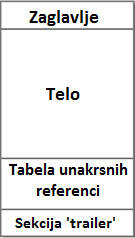
\includegraphics[width=0.2\textwidth]{pdfStruktura1_ispravljeno.png}
\caption{Структура датотека у формату \textit{PDF}}
\label{fig:pdfStruktura1}
\end{figure}

\begin{description}
\item \textbf{Заглавље} Прва линија датотеке чини њено заглавље и садржи број верзије формата \textit{PDF} која је коришћена у датотеци. У случају да се у датотеци налазе и бинарни подаци, потребно је у заглавље додати и другу линију која садржи најмање четири бинарна карактера (\textit{ASCII} вредност им је већа или једнака од 128). Друга линија служи као индикатор да се у датотеци налазе бинарни подаци, што је корисно апликацијама које раде са датотекама формата \textit{PDF}.
\item \textbf{Тело} Садржи све индиректне објекте који се налазе у датотеци.
Сви објекти су смештени у стабло, чији је корен објекат који се назива каталог објекат (енг. \textit{document catalog}). Каталог објекат је каталог који садржи информације о датотеци и реферише на друге објекте који дефинишу податке датотеке. 
Подстабло (стабла свих објеката) које садржи све објекте страница се назива \textit{стабло страница} (енг. \textit{page tree}). 
\item \textbf{Табела унакрсних референци} Табела \textit{xref} или табела \textit{cross reference} садржи податке о свим индиректним објектима у датотеци и омогућава брз приступ сваком од њих. Уместо претраге целе датотеке у потрази за одређеним објектом, локација објекта се прочита из табеле након чега му се може директно приступити.

Сваки објекат описан је једним редом у табели дужине 20 бајтова. Првих 10 бајтова имају различиту намену у зависности од врсте објекта. Постоје две врсте објеката: \textit{валидни} и \textit{ослобођени} објекти. Ове две врсте објеката, као и само ослобађање су објашњени у поглављу \ref{sec:azuriranje}. 

У случају валидног објекта, првих 10 бајтова садржи локацију објекта у датотеци. Локација објекта је одређена помоћу удаљености (енг. \textit{offset}) почетка датотеке до почетка дефиниције објекта. У случају ослобођеног објекта, првих 10 бајтова садржи број следећег ослобођеног објекта (референцу на следећи ослобођени објекат у повезаној листи свих ослобођених објеката).

Након првих 10 бајтова, у случају обе врсте објекта следи \textit{генерацијски број} (енг. \textit{generation/revision number}), који се увећава сваки пут када се објекат ослободи. Након генерацијског броја налази се индикатор који говори о врсти објекта: 'f' за ослобођен објекат или 'n' за валидан објекат. 
\item \textbf{"Trailer"} Ова секција датотеке се дефинише кључном речју \textit{trailer}. Овде се налази каталог који садржи информације о датотеци као нпр. број редова у табели унакрсних референци, референца на каталог објекат, итд. Најважнија информација је информација о локацији табеле унакрсних референци тј. о удаљености почетка датотеке до почетка дефиниције табеле. Број бајтова који представља удаљеност се наводи након кључне речи \textit{startxref}. Локација табеле је важна јер омогућава брз приступ табели, а она даље својом структуром омогућава брз приступ објектима датотеке. Последња линија секције \textit{trailer} садржи индикатор за крај датотеке $\%\%EOF$.
\end{description}

\section{Ажурирање датотека}
\label{sec:azuriranje}

Датотеке у формату \textit{PDF} се могу мењати, чиме се мења њихова структура тј. објекти у њима. Ажурирање датотеке не подразумева мењање оригиналног садржаја датотеке, већ додавање нових података на сам крај датотеке. Рецимо, заменом слике из датотеке новом сликом, објекат који представља стару слику неће бити обрисан или промењен тако да му садржај представља нову слику. Уместо тога, објекат старе слике биће означен као \textbf{ослобођен}, док ће објекат нове слике бити додат на сам крај датотеке. Тачније, ажурирањем датотеке се додаје ново тело, нова табела унакрсних референци и нова секција \textit{trailer} на крај датотеке. Ажурирање се може обављати неограничен број пута, при чему свака итерација (свако ажурирање) додаје три нове секције на крај датотеке. Датотека која је ажурирана $n$ пута је илустрована на слици \ref{fig:pdfStruktura2}. 

У новом телу се налазе нови или измењени објекти датотеке. Нова табела унакрсних референци садржи искључиво локације нових, измењених и ослобођених објеката. Локације старих објеката се и даље читају из старе табеле унакрсних референци (табеле унакрсних референци претходне итерације). До старих објеката се лако долази, јер нова секција \textit{trailer} поред локације нове табеле садржи и локацију претходне табеле. 

Сваки објекат који се обрише или измени постаје ослобођен, док се они који нису ослобођени називају \textit{валидни} објекти. Сви ослобођени објекти се налазе у једној повезаној листи. Они се третирају као обрисани и не могу бити у садржају датотеке, а референце на њих су једнаке објекту "Null". Ипак, објекат који је ослобођен може поново постати валидан неким наредним ажурирањем. \textit{Генерацијски број} објекта нам говори о укупном броју ослобађања једног објекта \cite{PDFDoc, introToPdf, basicStrPdf}.

Ажурирање датотеке на овај начин омогућава да се мале измене у великој датотеци брзо сачувају. Такође, некада је важно сачувати оригиналан садржај датотеке \cite{PDFDoc}.

\begin{figure}[t!]
\centering
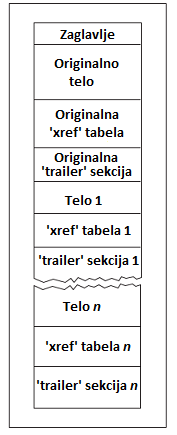
\includegraphics[width=0.3\textwidth]{pdfStruktura2.png}
\caption{Структура ажуриране датотекe у формату \textit{PDF}}
\label{fig:pdfStruktura2}
\end{figure}
% ------------------------------------------------------------------------------

% ------------------------------------------------------------------------------
\chapter{Имплементација програма за расплинуто тестирање читача датотека у формату \textit{PDF}}
\label{chp:implementacija}

Као демонстрација могућности Скале у паралелизацији задатака развијен је програм за расплинуто тестирање читача датотека у формату \textit{PDF}. Паралелизован је процес генерисања датотека у формату \textit{PDF}, као и њихово отварање у одређеном читачу. Програм користи библиотеку \textit{Akka} за имплементацију модела размене порука помоћу модела Aктер. Што се тиче самог тестирања, имплементиран је интелигентан тестер заснован на мутацијама. Мутације се примењују на садржај датотека из корпуса датотека, који је описан у наставку. Коришћена је верзија 2.12.5 језика Скала, а програм је развијен у окружењу \textit{IntelliJ IDEA Community Edition 2017.3.5}. Изворни к\^{о}д се налази у репозиторијуму на сајту \textit{github}\footnote{https://github.com/ancim/Master/tree/master/fuzzer}.

Корпус датотека је директоријум који садржи различитe датотекe у формату \textit{PDF}. Корисник може додавати и брисати датотеке из корпуса. Иницијално је у корпус смештено двадесет шест датотека. Све датотеке садрже типове објеката описане у поглављу \ref{sec:objektiPDF}, а оно што их разликује је садржај тих објеката и величина датотеке. Обухваћени су типови садржаја као што су текст, слике, аудио и видео записи, линкови, интерактивни дугмићи и тродимензионални објекти. 

\section{Улазни параметри}
\label{sec:ulazniParametri}

Покретањем програма са аргументом командне линије \textit{-{}-help} програм исписује упутство за корисника. Упутство садржи информације о аутору, сврси, начину рада и начину употребе програма. Пре почетка тестирања од корисника се тражи да унесе:
\begin{enumerate}
\item{\textbf{Читач датотека у формату \textit{PDF}}} који жели да тестира. Могуће је изабрати један од понуђених читача или унети путању до извршне датотеке произвољног читача.
\item{\textbf{Број итерација}} који представља број датотека који ће отворити сваки од објеката који су задужени за тестирање. Ти објекти су објекти Актер који су детаљно објашњени у наредном поглављу. % \ref{sec:actorObj}.  
\item{\textbf{Број објеката типа Извршилац}} који представљају објекте Актер који конкурентно (паралелно, уколико је могуће) мењају садржај датотека и отварају их у одабраном читачу. Ово су објекти класе \textit{Worker}, који су детаљније објашњени у поглављима \ref{sec:orgProg} и \ref{sec:actorObj}. Минималан број Извршилаца (објекте типа Извршилац ћемо у тексту звати краће Извршиоци) који корисник може да унесе је 1, а максималан зависи од рачунара на коме се извршава програм. Програм рачуна максималан број на основу два критеријума: броја језгара процесора и количине слободне меморије.

Уколико је број језгара процесора $x$, максималан број Извршилаца се најпре поставља на $3 \cdot x$. Иако истовремено не може радити више од $x$ Извршилаца, одабрано је да их буде више. Разлог томе је тај што сваки од њих након одређених акција чека да прође одређени број секунди (што је објашњено у поглављу \ref{sec:actorObj}). Како не би долазило до великог губљења времена док сви Извршиоци истовремено чекају, идеја је да их има више како би се извршавали конкурентно. Такође је важно да их не буде превише. Не треба  преоптеретити рачунар непотребним бројем објеката који се не могу паралелно извршавати јер нема довољно језгара. Превелики број објеката Актер може смањити перформансе због дељења много мањег броја процесора. Број $3$ је одабран експериментално.

Сваки Извршилац учитава целу датотеку у меморију. Због тога максималан број Извршилаца може бити и мањи од $3 \cdot x$: број се смањује уколико слободне меморије нема довољно да сваки од Извршилаца учита датотеку. Програм је подешен тако да дозвољава да датотеке заузимају половину слободне меморије.
\item{\textbf{Број милисекунди}} који представља време које се додељује читачу да отвори одређену датотеку. Неким читачима као што су \textit{Adobe}, \textit{Foxit} и \textit{Sumatra} довољно је 1000ms да отворе датотеку, док су неки други читачи као што је читач \textit{Slim} много спорији и потребно им је барем 3000ms. Уколико се читачу не додели довољан број секунди за отварање датотеке, процес задужен за отварање ће бити угашен пре него што је датотека отворена. У том случају програм неће успети да детектује грешку у читачу (уколико она постоји). Због тога је најбоље пре самог тестирања читача проценити отприлике који број милисекунди му је довољан за отварање датотека.
\end{enumerate}

Пре тестирања одређеног читача потребно је подесити га тако да сваку датотеку отвара у посебном процесу. То се код многих читача постиже тако што се одабере опција да се свака датотека отвара у новом прозору  (уколико та опција није подразумевана). На тај начин раде читачи који су тестирани у овом раду. Ипак, нови прозор не представља нужно и нови процес, због чега је увек потребно проверити на који начин ради одређени читач. Један од начина на који се то може проверити је излиставање и посматрање активних процеса у командној линији. Отварање сваке датотеке у посебном процесу је неопходно за правилан рад програма. Уколико неки читач не дозвољава такав начин рада, он не може бити тестиран имплементираним програмом. 

\section{Организација програма}
\label{sec:orgProg}

Програм је организован у четири класе које су приказане дијаграмом на слици \ref{fig:classDiagram}. Класе \textit{Controler} и \textit{Worker} представљају објекте Актер задужене за паралелизацију тестирања. Способност \textit{Timers} је спојена у класу \textit{Worker}, а класа \textit{ParserPDF} је задужена за мутацију садржаја датотека. Главни програм налази се у објекту \textit{actors} који представља једини објекат истоимене класе. Због тога се он означава као објекат \textit{singleton}. У наредним поглављима је детаљније приказан начин рада објеката ових класа. 

\begin{figure}[!ht]
  \centering
  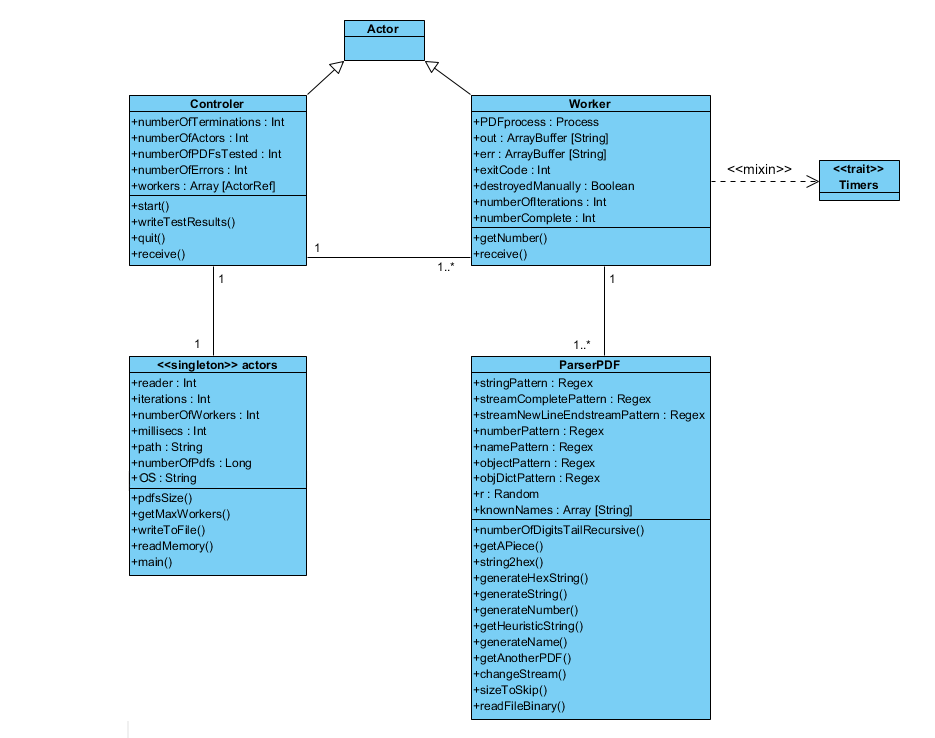
\includegraphics[width=1\textwidth]{classDiagram.png}
  \caption{Дијаграм класа}
  \label{fig:classDiagram}
\end{figure}

\section{Oбјекти Актер}
\label{sec:actorObj}

Сви објекти Актер у програму припадају једном систему \textit{ActorSystem}. На врху хијерархије корисничких компоненти налази се један објекат Актер класе \textbf{Controler} који је задужен за покретање и праћење рада свих осталих објеката Актер. Њега називамо \textit{Контролер}. Систем \textit{ActorSystem} и објекат Контролер се креирају у функцији \textit{main} која се налази у објекту \textit{actors}. Њихово креирање и слање поруке објекту Контролер је приказано у следећем примеру:

\begin{lstlisting}[frame=single]
     val system = ActorSystem("fuzzerSystem");
     val a = system.actorOf(Props[Controler], name="fuzzer-controler-actor")
     a ! "Pocni!";
\end{lstlisting}

Објекат Контролер креће са радом када прими поруку "Pocni!". Тада позива метод \textit{start()}, који је приказан у следећем сегменту кода:

\begin{lstlisting}[frame=single]
    def start() = {
        println("Pokrecem Worker-e");
        val workers: Array[ActorRef] = new Array[ActorRef](numberOfActors);
        for(i <- 0 until numberOfActors) {
            /* pravimo Actor-a i saljemo mu poruku za pokretanje */
            workers(i) = context.actorOf(Props(new Worker(i, numberOfActors)), name = "myWorker-" + i);
            context.watch(workers(i));
            workers(i) ! "Pokreni";
        }
    }
\end{lstlisting}

Објекат Контролер генерише друге објекте Актер који су објекти класе \textbf{Worker}. Као што је поменуто у поглављу \ref{sec:ulazniParametri}, њих називамо \textit{Извршиоци}. Контролер чува референце на Извршиоце (типа \textit{ActorRef}) у низу, и сваком од њих шаље поруку за покретање (порука "Pokreni"). Метод \textit{watch} омогућава Контролеру да "посматра" креиране Извршиоце, што значи да ће бити обавештен сваки пут када неки од њих заврши са радом.

Извршиоци су објекти који су задужени за примену расплинутог тестирања. Сваки од њих има свој редни број на основу кога учитава једну од датотека из корпуса датотека. Извршиоци садрже објекат класе \textbf{PDFparser}, који примењује мутације над подацима те датотеке, како је описано у поглављу \ref{sec:kreiranjeDat}. На тај начин Извршилац добија тест пример тј. нову датотеку коју треба да отвори у читачу који се тестира.
 
Отварање измењене датотеке се догађа у спољашњем процесу чије се извршавање може надзирати. То се постиже помоћу библиотеке \textit{scala.sys.process}. Ова библиотека омогућава извршавање, посматрање спољашњег процеса и руковање његовим улазом и излазом. Основу ове библиотеке чине класе \textit{Process} и \textit{ProcessBuilder} језика Јава. Скала има класе истих имена и оне су коришћене у имплементацији.

Претпоставка је да сваки читач треба да препозна лоше конструисане и злонамерне датотеке, да пријави грешку и нормално настави са радом. У случају да се читач сам угаси након отварања датотеке, то је индикатор да је дошло до грешке коју није умео да обради. Због тога се спољашњем процесу који покреће читач даје одређено време (улазни параметар \textit{број милисекунди} наведен у поглављу \ref{sec:ulazniParametri}) да отвори датотеку, након чега се анализира његово стање. Уколико је процес и даље активан, то значи да је датотека и даље отворена у читачу или да је читач успешно обрадио грешку насталу при отварању. Тада се овај процес прекида од стране Извршиоца који га је креирао. Са друге стране, уколико процес није активан, то значи да се сам угасио и да је пронађена слабост читача. У том случају се документују стандардни излаз, стандардни излаз за грешке и повратна вредност процеса. То су информације о извршавању процеса. Ове информације се чувају у текстуалној датотеци у директоријуму "results". Назив текстуалне датотеке садржи префикс "CRASH\_" након кога следи редни број Извршиоца. Такође, поред префикса "CRASH\_" могу следити и префикси "ERR\_" и "NULL\_". Префикс "ERR\_" се појављује уколико стандардни излаз за грешке није празан, а "NULL\_" уколико је нека од информација о процесу \textit{NULL}. Чува се и датотека која је узроковала грешку, у директоријуму "fuzzedPDFError".

Команда која отвара датотеку која се налази у директоријуму "fuzzedPDFcorpus" у читачу \textit{SlimPDFReader} и покретање спољашњег процеса приказани су у следећем примеру:

\begin{lstlisting}[frame=single, language=Scala]
    val command = ".\\PDF_citaci\\slim\\SlimPDFReader.exe .\\fuzzedPDFcorpus\\" + numberComplete +               "_fuzzed.pdf";
    /* za nekoliko sekundi saljemo poruku "stop" sami sebi kako bismo analizirali stanje procesa */
    timers.startSingleTimer("key", "stop", millisecs milliseconds);

    /* pokretanje spoljasnjeg procesa */
    val qb: ProcessBuilder = Process(command)
    PDFprocess = qb run (ProcessLogger((s) => { out ::= s},
	    					        (s) => { err ::= s}));
\end{lstlisting}

Команда која отвара датотеку је дата као ниска карактера облика: ".\textbackslash odabranCitac.exe .\textbackslash nazivDatoteke.pdf". Чекање од одређеног броја милисекунди пре анализирања статуса процеса се остварује помоћу способности \textit{akka.actor.Timers} који садржи објекат \textit{timers} апстрактне класе \textit{TimerScheduler}. Метод \textit{startSingleTimer} овог објекта омогућава Извршиоцу да сам себи пошаље поруку у одређено време тј. након дефинисаног броја секунди. Као што се види у примеру, објекат ће након \textit{millisecs} милисекунди себи послати поруку "stop". Када Извршилац прими поруку "stop", то значи да је истекао период рада спољашњег процеса. Тада Извршилац треба да анализира  статус процеса и да га заустави уколико је још увек активан. Класе \textit{Process} и \textit{ProcessBuilder} се користе за креирање процеса на основу дате команде. Метод \textit{run} извршава дати процес, а њему се прослеђује објекат типа \textit{ProcessLogger} који рукује стандардним излазом и стандардним излазом за грешке. Стандардни излаз се уписује у листу ниски карактера \textit{out}, а стандардни излаз за грешке у листу ниски карактера \textit{err}.

Извршиоци се извршавају конкурентно (или паралелно) и изнова креирају тест примере и нове спољашње процесе који их отварају у читачу. Број датотека које ће креирати и отворити сваки од њих зависи од \textit{броја итерација} који је унео корисник пре почетка тестирања. Једна итерација подразумева да сваки Извршилац тестира читач отварањем једне датотеке. На пример, ако желимо да сваки Извршилац отвори $x$ датотека, треба да унесемо $x$ као број итерација. Укупан број датотека које ће програм отворити у читачу је онда $n \cdot x$, где је $n$ број Извршилаца. Друга могућност је да се програм извршава све док корисник сам не прекине извршавање програма. У том случају, као број итерација треба унети број $-1$.

Уколико је дефинисан одређени број итерација (ако је различит од $-1$), сваки Извршилац завршава са радом када анализира последњи процес који је покренуо. Тада зауставља сам себе, а порука о томе се шаље његовом супервизору, објекту Контролер. Када Контролер добије поруку о заустављању од сваког детета, он зауставља цео систем \textit{ActorSystem} чиме се завршава извршавање програма.

Интеракција објеката приказана је дијаграмом комуникације на слици \ref{fig:dijagramKomunikacije}. Како број Извршилаца зависи од уноса корисника и рачунара на ком се извршава програм, на дијаграму је приказан само један Извршилац и његова комуникација са другим објектима. Такође, приказ више Извршилаца на дијаграму је незгодан због паралелизма и конкурентности у програму. Не можемо предвидети када ће одређени Извршилац добити процесорско време, због чега је немогуће приказати тачан редослед корака и порука које објекти размењују. Оно што се може одредити и што је приказано на дијаграму јесу кораци кроз које пролазе сви Извршиоци. Важно је напоменути и да Извршиоци не комуницирају између себе.  

\begin{figure}[!ht]
  \centering
  \frame{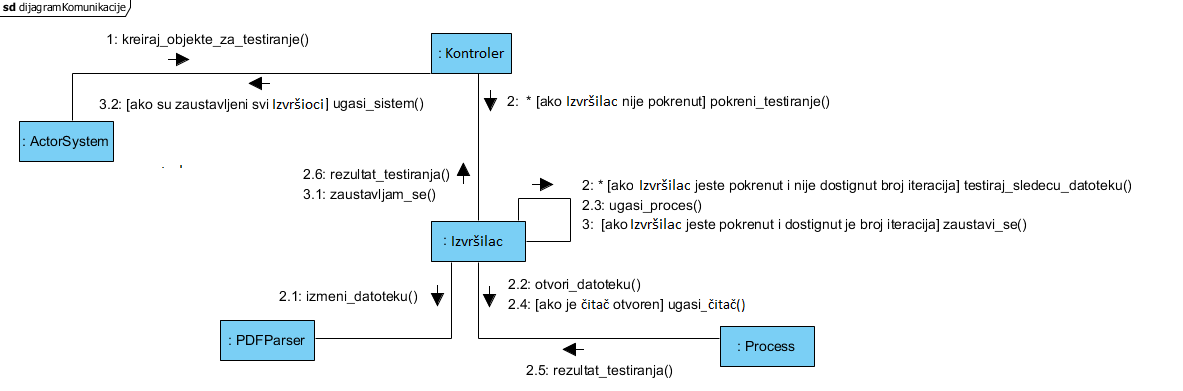
\includegraphics[width=1\textwidth]{dijagramKomunikacije.png}}
  \caption{Дијаграм комуникације}
  \label{fig:dijagramKomunikacije}
\end{figure}

\section{Креирање датотека у формату \textit{PDF}}
\label{sec:kreiranjeDat}

Објекти класе \textbf{ParserPDF} су објекти који примењују измене над садржајем датотеке коју добију као аргумент. Ова датотека представља улаз тј. основу за конструисање нове датотеке. Применом мутација над неким подацима постојеће датотеке добија се нова датотека која ће бити коришћена као тест пример. 

Због присуства бинарних података у датотекама формата \textit{PDF}, садржај целе датотеке се најпре учитава као низ бајтова. Низ бајтова се потом конвертује у ниску карактера, јер је потребно претражити садржај датотеке у облику разумљивом људима. Ниска карактера се претражује у потрази за објектима одређених типова, ради њихове измене. Када се измени жељени садржај, потребно је ниску карактера конвертовати натраг у низ бајтова који ће бити уписан у нову датотеку. При обе конверзије је важно користити једнобајтну кодну шему \textit{ISO-8859-1}. Ова кодна шема је погодна јер чува оригиналан садржај бинарних података. Наиме, 
у вишебајтним кодним шемама није свака секвенца бајтова валидна, због чега се при декодирању секвенце она може пресликати у неки заменски карактер (нпр. ? или \quem). То се може догодити током конверзије низа бајтова у ниску карактера. На основу ових заменских карактера је немогуће добити натраг полазну секвенцу бајтова (при конверзији ниске карактера натраг у низ бајтова). Такође, неке једнобајтне кодне шеме не кодирају свих 256 различитих карактера. Због тога је у овом случају потребно користити једнобајтно кодирање које кодира 256 различитих карактера. На тај начин се бајтови јединствено пресликавају у карактере, а касније се ти карактери јединствено пресликавају у бајтове.

Када је датотека претворена у ниску карактера, тада се део њеног садржаја мутира тј. мења. Мутације се примењују над различитим типовима објеката датотеке: бројевима, нискама карактера, именима, индиректним објектима, каталозима и токовима. Због тога је потребно препознати појављивања ових објеката у датотеци. Треба напоменути да се унутар токова игнорише појављивање било ког другог објекта јер токови садрже бинарне податке које не треба претраживати као ниске карактера. Препознавање објеката се врши помоћу \textit{регуларних израза}. 
%Пребројавање је важно јер се на основу броја појављивања одређеног објекта одређује број објеката чија ће вредност бити промењена. Број података који се мења се одређује случајно, али тако да буде мали у односу на укупан број података. Идеја је преварити програм задржавајући велики број валидних података, како би се смањила вероватноћа да програм одмах одбаци датотеку.
%
Библиотека која омогућава коришћење регуларних израза у Скали је библиотека \textit{scala.util.matching}. Регуларни изрази су дефинисани на следећи начин:

\begin{lstlisting}[frame=single]
    /* sabloni koje pretrazujemo u datotekama */
  val stringPattern: Regex = """\([\s\S]+?\)|\<[0-9a-fA-F]*?\>""".r
  val streamCompletePattern: Regex = """(stream)([\s\S]+?)(endstream)""".r
  val streamNewLineEndstreamPattern: Regex = """(stream)\n(endstream)""".r
  val numberPattern: Regex = """[+-]?((\d+\.?\d+)|(\d*\.?\d+)|(\d+\.?\d*))""".r
  val namePattern: Regex = """/[a-zA-Z0-9]+""".r
  val objectPattern: Regex = """(\d+) (\d+) (obj)([\s\S]+?)(endobj)""".r
  val objDictPattern = """(obj)([\s]*)(<<)([\s\S]+?)(>>)""".r    
\end{lstlisting}

Применом метода \textit{r} на ниске карактера које представљају регуларне изразе добијамо обрасце који су типа \textit{scala.util.matching.Regex}.

Следећи пример илуструје: читање и смештање бајтова датотеке у низ бајтова, конверзију низа бајтова у ниску карактера, и проналажење свих токова података у ниски карактера помоћу обрасца \textit{streamCompletePattern} (који је дефинисан у претходном примеру):

\begin{lstlisting}[frame=single]
    val byteArray: Array[Byte] = Files.readAllBytes(Paths.get(fileName));
    /* pravimo string koji sadrzi podatke iz datoteke */
    var contentString = new String(byteArray, Charset.forName("ISO-8859-1"))
    val matchStreams = streamCompletePattern.findAllMatchIn(contentString).toList
\end{lstlisting}

Подаци се читају из датотеке чија је путања наведена у ниски карактера \textit{fileName}. Коришћена је библиотека \textit{java.nio.file} и њена класа \textit{Files} која садржи различите статичке методе за манипулацију датотекама и директоријумима. Метод \textit{readAllBytes} чита бајтове датотеке који се чувају у низу бајтова \textit{byteArray}. Од добијеног низа бајтова се конструише ниска карактера \textit{contentString}. Метод \textit{findAllMatchIn} проналази сва појављивања регуларног израза у ниски карактера, а метод \textit{toList} сва појављивања смешта у листу.

Радње које се примењују над објектима које треба изменити су брисање, додавање и измена постојећих података, при чему се над једним објектом не морају применити све радње. На пример, неке објекте можемо заменити новим објектом истог типа, док неке друге можемо добити брисањем једног дела садржаја објекта. Нови објекти могу бити исте или различите величине од објекта који мењају. Могу се  добити псеудо случајно или помоћу хеуристика. 

Генерисање псеудо случајних података се врши методама класе \textit{scala.util.Random}. На пример, псеудо случајан цео број се може добити позивом метода \textit{Random.nextInt()}. Слично, постоје и методе \textit{Random.nextString()}, \textit{Random.nextDouble()}, итд. 

Што се тиче хеуристика, коришћен је приступ који у своје тест примере умеће вредности објеката које често доводе до грешака у раду програма. Типови објеката који су обухваћени су ниске карактера, цели и реални бројеви. Вредности ових типова су прикупљене са два репозиторијума на сајту \textit{github}\footnote{https://github.com/minimaxir/big-list-of-naughty-strings/tree/master/naughtystrings}\footnote{https://github.com/fuzzdb-project/fuzzdb/tree/master/attack}. Ови репозиторијуми садрже податке који имају велику вероватноћу да изазову разне врсте грешака када се користе као улазни подаци програма. Ту се могу наћи адекватни улазни подаци у зависности од типа улазних података, природе програма који се тестира и типичних врста напада на програм, оперативног система на коме се извршава програм, итд. Нова вредност објекта који се мења хеуристички ће бити случајно одабрана из свих прикупљених вредности тог типа.

Прва измена која се примењује над датотекама је брисање неких индиректних објеката. Број објеката и објекти који ће бити обрисани се одређују случајно, након чега је датотека спремна за претраживање осталих типова објеката.
У наставку су објашњени могући начини њихове измене:
\begin{description}
\item{\textbf{Бројеви}} При измени бројa случајно се одређује начин на који ће се генерисати нови број који ће га заменити: псеудослучајно или помоћу хеуристика. Прикупљених бројева има мало и то су граничне вредности (целих и реалних бројева), вредности блиске нули, бројеви $0$, $-1$, итд. Ови бројеви често изазивају грешке прекорачења меморије. У малом броју случајева, број се мења хеуристички изабраном ниском карактера. 

Поред токова података и имена, објекти који се највише појављују у датотекама формата \textit{PDF} су бројеви. Они су распрострањени свуда, а највише као идентификатори других објеката. Мењањем референци на друге објекте можемо постићи реферисање на непостојеће, невалидне или објекте погрешног типа.  
\item{\textbf{Ниске карактера}} При измени ниске карактера случајно се одређује један од три начина измене. Прва два начина су једнака као и код измене бројева: псеудослучајно или хеуристички. Дужине псеудослучајних ниски карактера се одређују случајно тако да некад буду једнаке као ниске карактера које мењају, а некад им се дужина одреди случајно. Што се тиче хеуристика, прикупљених ниски карактера има јако много, а неки примери су приказани у табели \ref{table:niske}. Најчешће ниске које се користе за тестирање су ниске карактера са описом формата, ниске које представљају претрагу по систему датотека, ниске које садрже специјалне карактере, позиве функција, \textit{html} тагове, итд. Трећи начин мења ниску карактера ниском која представља целу датотеку формата \textit{PDF}. Циљ је уметнути другу датотеку у датотеку чији садржај мењамо. Датотека која се умеће може бити исправна датотека или датотека коју је раније "покварио" тј. генерисао програм за тестирање.
\item{\textbf{Имена}} При измени имена случајно се одређује један од три начина измене. Први начин генерише име псеудослучајно тј. ниску карактера која почиње знаком '/' за којим следи ниска карактера произвољне дужине. Други начин уместо имена умеће хеуристички одабрану ниску карактера, док трећи начин представља замену имена једним од имена који се често користе у датотекама формата \textit{PDF}. Често коришћена имена су дефинисана у самом програму и прикупљена су на основу корпуса датотека.
\item{\textbf{Токови података}} Објекти овог типа се не могу мењати као обичне ниске карактера већ се конвертују у низ бајтова. Како су токови података већином веома дугачки, није циљ променити цео ток већ променити само његове "парчиће". "Парчићи" су његови поднизови који најчешће буду промењени псеудо случајним низовима бајтова добијеним методом \textit{Random.nextByte()}. У малом броју случајева, подниз буде замењен низом бајтова који представља другу датотеку (уметање друге датотеке је могуће и код измене ниске карактера). Број поднизова за измену, њихова величина и локација у низу се одређују случајно. Након свих промена у низу бајтова, он се конвертује натраг у ниску карактера. При свакој конверзији користи се кодна шема \textit{ISO-8859-1}. 
\item{\textbf{Каталози}} Каталози који се могу променити у датотеци су каталози који следе након дефиниције индиректних објеката, тј. након кључне речи \textit{obj}. Они се одређују случајно и мењају се на само један начин: сваки каталог одабран за промену копира садржај претходно одабраног каталога (у случају првог одабраног каталога, његов садржај остаје непромењен). 
\end{description}

\begin{table}
    \begin{tabular}{| p{14cm} |}
    \hline
%    \thead{Ниска карактера} & \thead{Опис}  \\ \hline
    System(\textbackslash''ls -al /\textbackslash'') \\ \hline
    <?xml version=\textbackslash''1.0\textbackslash'' encoding=\textbackslash''ISO-8859-1\textbackslash''?><!DOCTYPE foo [ <!ELEMENT foo ANY ><!ENTITY xxe SYSTEM \textbackslash''file:///etc/passwd\textbackslash'' >]><foo>\&xxe;</foo> \\ \hline
	\$ENV\{'HOME'\}\\ \hline
	../../../../../../../../../../../etc/passwd\%00\\ \hline
	Kernel.exec(\textbackslash''ls -al /\textbackslash'')\\ \hline
	eval(\textbackslash''puts 'hello world'\textbackslash'')\\ \hline
	1'; DROP TABLE users-- 1\\ \hline
	</textarea><script>alert(123)</script>\\ \hline
	<IMG SRC=\textbackslash''javascript:alert('XSS')\textbackslash''\\ \hline
	/..\%c1\%9c..\%c1\%9c..\%c1\%9c..\%c1\%9c..\%c1\%9c\{FILE\}\\ \hline
	/../../../../../../../../\{FILE\}\\ \hline
    	DCC SEND STARTKEYLOGGER 0 0 0 \\ \hline
\%d\%d\%d\%d\%d\%d\%d\%d\%d\%d\%d\%d\%d\%d\%d\%d\%d\%d\%d\%d\%d\%d\%d\%d \\ 
\%d\%d\%d\%d\%d\%d\%d\%d\%d\%d\%d\%d\%d\%d\%d\%d\%d\%d\%d\%d\%d\%d\%d\%d \\
\%d\%d\%d\%d\%d\%d  \\
    	\hline
    \end{tabular}
\caption{Примери ниски карактера}
\label{table:niske}
\end{table}

\section{Резултати тестирања}
\label{sec:rez}

У току тестирања читача долазило је до проблема са недостатком меморије. Због тога су одређени делови кода имплементирани на два начина, због чега разликујемо прву и другу верзију програма. У наставку су описане обе верзије, њихово поређење и грешка која се јављала.

Приликом тестирања прве верзије програма дешавало се да програм избаци изузетак: \textit{java.lang.OutOfMemoryError: Java heap space}. До овог изузетка долази када Јава виртуелна машина нема довољно слободне хип меморије. Оно што је било збуњујуће при појављивању ове грешке је што се она манифестовала веома непредвидиво: некад након три сата рада програма, некад након десет минута, а некада се није ни манифестовала. Честим исписивањем количине слободне хип меморије заиста се видело да се у неким случајевима меморија редовно ослобађа, док у другима након одређеног времена количина слободне меморије пада све док се не деси избацивање изузетка. Овакво понашање упућивало је на цурење меморије које се не манифестује увек.

Експлицитно постављање референци објеката на \textit{null}, и иницирање сакупљача отпадака из програма није помогло, тако да је наредни корак био покретање програма заједно са профајлером \textit{VisualVM}. Профајлер омогућава лакше и јасније праћење рада програма и меморије, нарочито исписивањем алоцираних објеката у меморији када се деси изузетак. 

На сликама \ref{fig:monitor} и \ref{fig:HD} приказан је пример рада програма у профајлеру. За улазне параметре постављени су читач \textit{Sumatra}, број $-1$ као број итерација, број $10$ као број Извршилаца и број $1000$ као број милисекунди. Прва слика приказује целокупан рад програма. Од посебне важности је секција \textit{Heap} коју чини график који приказује количину слободне хип меморије у зависности од времена. Може се видети да је програм радио преко три сата, редовно ослобађајући меморију све док у једном тренутку количина меморије није нагло порасла до границе коју дозвољава Јава виртуелна машина. Када је избачен изузетак, забележени су објекти алоцирани на хипу, што је приказано на другој слици. Највећи део меморије заузимају инстанце класе \textit{scala.collection.immutable.\$colon\$colon}, која представља непроменљиве листe у Скали. Програм је у једном тренутку заузео меморију великом количином листи чији је тип елемената био \textit{Regex.Match} (што је такође прочитано из профајлера). Објекти овог типа представљају појављивања одређених регуларних израза. Регуларни изрази  омогућавају претраживање различитих објеката у датотеци (како је објашњено у поглављу \ref{sec:kreiranjeDat}).

\begin{figure}[t!]
\centering
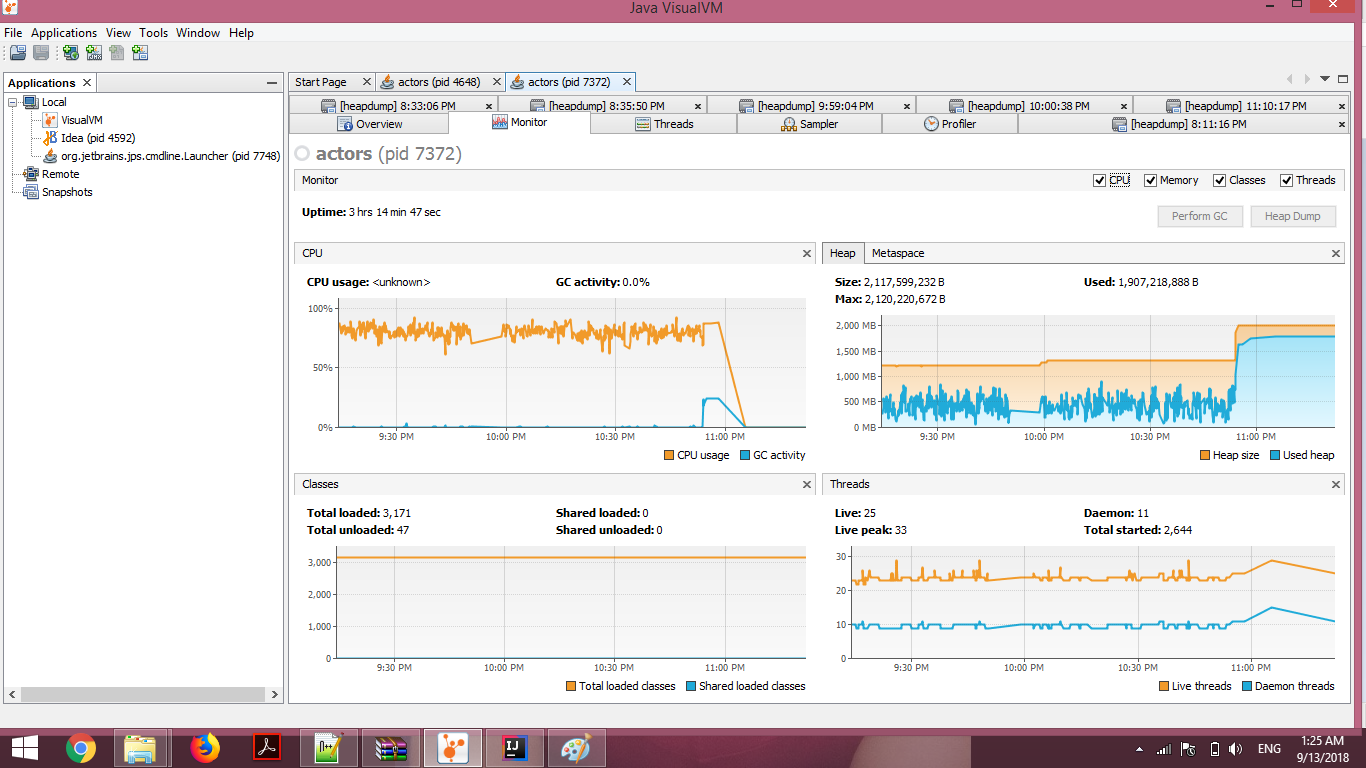
\includegraphics[width=1\textwidth]{10_Workera_1000ms.png}
\caption{Приказ рада програма помоћу профајлера \textit{VisualVM}}
\label{fig:monitor}
\end{figure}

\begin{figure}[t!]
\centering
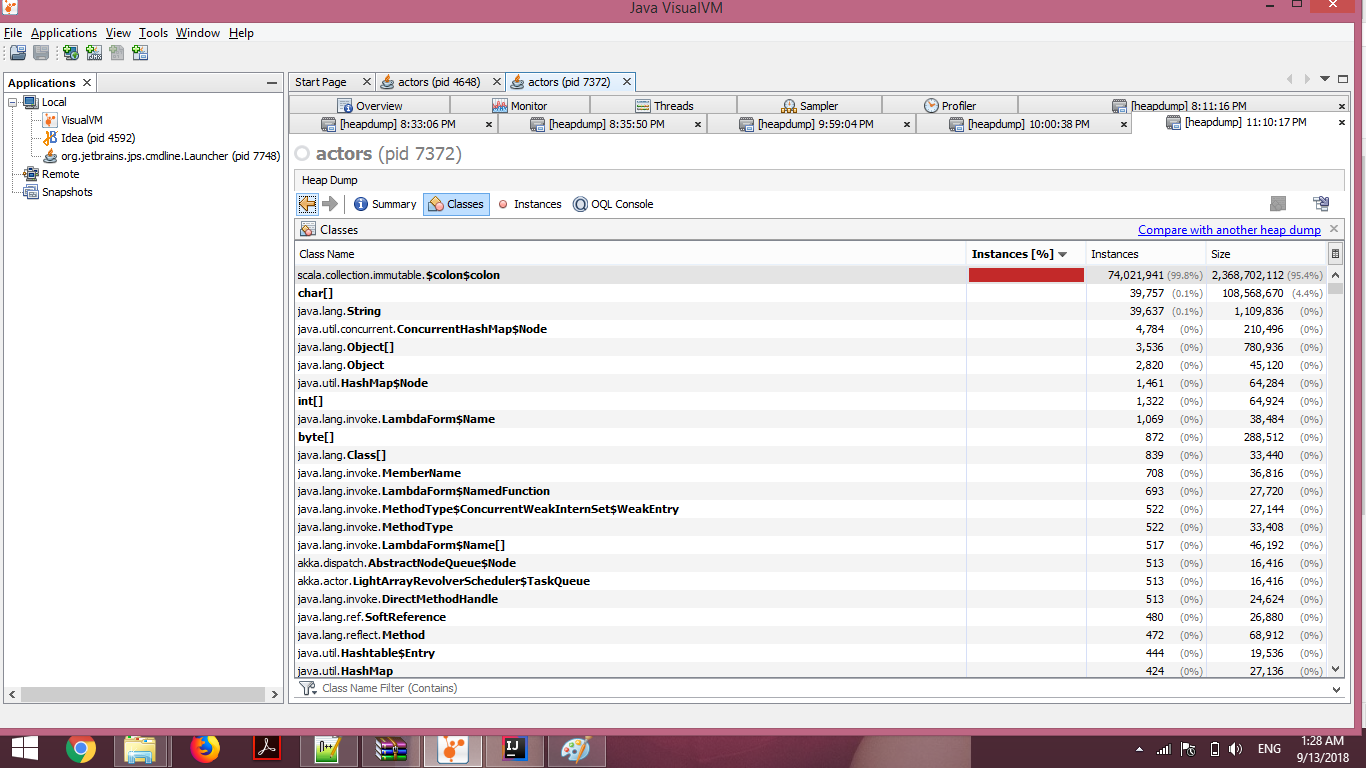
\includegraphics[width=1\textwidth]{10_Workera_1000ms_HD6.png}
\caption{Приказ алоцираних објеката помоћу профајлера \textit{VisualVM}}
\label{fig:HD}
\end{figure}

Начин на који је имплементирано претраживање и мењање објеката у првој верзији програма је могао бити разлог преоптерећења меморије листама. Тај начин је подразумевао да се сваки тип објекта у датотеци претражује функцијом \textit{scala.util.matching.Regex.findAllMatchIn}, која проналази \textbf{сва} појављивања одговарајућег регуларног израза. Сва појављивања су смештана у листу, након чега се на основу броја појављивања бирао јако мали број објеката који ће бити промењени. Када је завршено са свим променама објеката, листа која садржи појављивања је постављена на \textit{null}. Разлог недостатка меморије је могао бити тај да су листе биле превелике да би стале у меморију уколико је број појављивања одређених објеката био превелик. Такође, због конкурентности у програму, могло се десити да више нити у исто време захтева чување великих листи у меморији. 

Друга верзија програма је имплементирана тако да избегне конструкцију и чување листи. Уместо претраживања свих појављивања објеката одједном, појављивања су тражена и чувана једно по једно. Коришћена је функција \textit{scala.util.matching.Regex.findFirstMatchIn} која проналази само \textbf{прво} појављивање регуларног израза тј. објекта. Када се пронађени објекат промени, случајно одређени део датотеке се прескаче, након чега се одатле поново тражи прво појављивање објекта одређеног типа. Тај поступак се понавља све до краја датотеке. На тај начин свака нит у меморији чува само по један, тренутно пронађени објекат.

Ипак, друга верзија програма није исправила грешку недостатка меморије. Грешка о недостатку хипа је наставила непредвидиво да се манифестује, појављујући се након различитог периода рада програма. Највећи део заузете хип меморије су и даље биле листе типа \textit{Regex.Match}, иако у имплементацији не постоји део кода за који се може претпоставити да генерише овакве листе. Због тога се претпоставља да је проблем у структурама података које се користе за функционални део Скале.

Због грешке недостатка меморије тешко је упоредити прву и другу верзију програма. Тестирањем друге верзије није се видело побољшање, али се јасно поређење не може дати са сигурношћу због непредвидивог понашања обе верзије. Друга верзија захтева више времена за обраду једне датотеке, што није значајно у случају мањих датотека, док је у случају већих датотека разлика приметна.

Иако проблем није отклоњен, обе верзије програма су неко време тестирале читаче и постигле одређене резултате. Тестирана су три читача: \textit{Foxit}, \textit{Sumatra} и читач \textit{Slim}. Одабрани су мање познати читачи због претпоставке да су мање отпорни на грешке од познатијих читача као што је читач  \textit{Adobe}. Ниједна верзија програма није успела да пронађе грешку у читачима \textit{Foxit} и \textit{Sumatra}. Оба читача су успешно препознала сваку неисправну датотеку пријављујући грешку при отварању. Са друге стране, читач \textit{Slim} се показао као веома слаб. Обе верзије програма су често изазивале грешке у његовом раду. Један начин на који је читач \textit{Slim} показао слабост је гашење одмах при отварању неисправне датотеке. Обе верзије програма су детектовале овакво понашање и сачувале датотеке које су изазвале гашење читача. Други начин на који је читач \textit{Slim} показао неправилно понашање је престанак реаговања након отварања датотеке. У том случају оперативни систем издаје обавештење да је читач престао да реагује. Програм то не успева да детектује јер је у том случају спољашњи процес који је задужен за отварање датотеке и даље активан.

Такође је важно напоменути да обе верзије програма пријављују грешке код читача \textit{Slim} и онда када он ради како треба. Узрок томе је карактеристика читача \textit{Slim} која је присутна и код читача \textit{Adobe}. Наиме, оба читача гасе покренуту инстанцу читача када препознају неисправну датотеку, и издају обавештење о неисправној датотеци. Због тога што сами угасе инстанцу читача, програм то детектује као да је процес угашен због проналаска грешке. Зато је при тестирању читача \textit{Slim}, за сваку пронађену неисправну датотеку потребно ручно проверити да ли заиста изазива грешку читача. Читаче са оваквим начином рада није погодно тестирати имплементираним програмом, али је у овом раду читач \textit{Slim} ипак тестиран јер је пронађено доста правих грешака. 


%\begin{figure}[t!]
%\centering
%\includegraphics[width=1\textwidth]{4_Workera_1200ms.png}
%\caption{Приказ рада програма помоћу профајлера VisualVM}
%\label{fig:pokretanjeWorkera}
%\end{figure}

%Тестирање је примењено на PDF читаче Foxit

%
%\begin{figure}[t!]
%\centering
%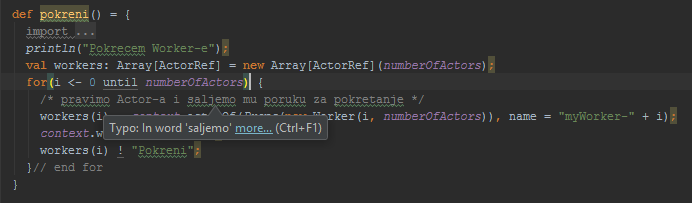
\includegraphics[width=1\textwidth]{pokretanjeWorker-a.png}
%\caption{Генерисање и покретање Actor објеката}
%\label{fig:pokretanjeWorkera}
%\end{figure}


% ------------------------------------------------------------------------------

% ------------------------------------------------------------------------------
\chapter{Закључак}
\label{chp:zakljucak}

%У овом раду описанe су карактеристике програмског језика Скала због којих је она погодна за решавање %разних проблема а посебно оних који захтевају конкурентно и паралелно извршавање.

Због великих потреба за паралелним извршавањем веома је важно упознати нове технологије, језике и библиотеке које се развијају како би олакшале развој захтевних програма. Зато су представљена функционална својства Скале и начин на који се у њој може имплементирати модел Актер помоћу библиотеке \textit{Akka}. Идеја којa стоји иза овог модела и поменута библиотека су се показале као веома интуитивне и лагане за рад. Имплементиран је програм који конкурентно и паралелно тестира читаче датотека у формату \textit{PDF} помоћу технике расплинутог тестирања. Концепт размене порука је омогућио брзу и лаку имплементацију паралелизације. 

Приликом расплинутог тестирања се за генерисање улазних параметара некад користе специфичне вредности, али генерално не постоје правила по којима се они генеришу. Због тога ова техника тестирања омогућава развој креативности и даје слободу програмеру. У овом раду су покретани читачи датотека са датотекама чији је садржај претходно измењен у програму. 

Један од изазова који су карактеристични за конкурентно и паралелно изавршавање је детектовање и исправљање грешака. Грешке које се појављују у конкурентним и паралелним програмима се често манифестују непредвидиво што се показало и у овом раду. Приликом извршавања програма за тестирање читача датотека је у различитим тренуцима долазило до недостатка хип меморије. Било је веома тешко открити узрок овакве грешке, тако да је било потребно извршавати програм уз помоћ профајлера. Профајлер је показао резултате који су показали да се узрок овакве грешке највероватније налази у имплементацији неких од метода Скалине библиотеке за рад са регуларним изразима.

Такође се показало и да није лако изазвати грешке у раду читача датотека. На интернету се брзо може доћи до разних познатих напада на програме тако да је већина данашњих читача доста јака и отпорна на нападе. Потребно је много истраживања, времена и труда за откривање грешака у њима. У раду су за тестирање одабрана три мање позната читача од којих се један показао као веома слаб јер је доста често престајао са радом. 

Датотеке у формату \textit{PDF} су веома комплексне и њихово дубље проучавање представља највећи простор за побољшање имплементираног програма. Бољим парсирањем датотека и мењањем њихових објеката на више начина постоје веће шансе за проналазак грешака у читачима. Програм се може побољшати и тако да омогући: детектовање престанка реаговања читача, покретање читача уз дибагер, мењање датотека без учитавања целог њиховог садржаја одједном, итд. 

% ------------------------------------------------------------------------------

% ------------------------------------------------------------------------------
% Literatura
% ------------------------------------------------------------------------------
\literatura

% ==============================================================================
% Završni deo teze i prilozi
\backmatter
% ==============================================================================

% ------------------------------------------------------------------------------
% Biografija kandidata
%\begin{biografija}
%\textbf{Вук Стефановић Караџић} (\emph{Тршић, 26. октобар/6. новембар
%  1787. — Беч, 7. фебруар 1864.}) био је српски филолог, реформатор
%српског језика, сакупљач народних умотворина и писац првог речника
%српског језика.  Вук је најзначајнија личност српске књижевности прве
%половине XIX века. Стекао је и неколико почасних доктората.
%Учествовао је у Првом српском устанку као писар и чиновник у
%Неготинској крајини, а након слома устанка преселио се у Беч,
%1813. године. Ту је упознао Јернеја Копитара, цензора словенских
%књига, на чији је подстицај кренуо у прикупљање српских народних
%песама, реформу ћирилице и борбу за увођење народног језика у српску
%књижевност. Вуковим реформама у српски језик је уведен фонетски
%правопис, а српски језик је потиснуо славеносрпски језик који је у то
%време био језик образованих људи. Тако се као најважније године Вукове
%реформе истичу 1818., 1836., 1839., 1847. и 1852.
%\end{biografija}
% ------------------------------------------------------------------------------

\end{document} 